% Options for packages loaded elsewhere
\PassOptionsToPackage{unicode}{hyperref}
\PassOptionsToPackage{hyphens}{url}
\documentclass[
]{book}
\usepackage{xcolor}
\usepackage{amsmath,amssymb}
\setcounter{secnumdepth}{5}
\usepackage{iftex}
\ifPDFTeX
  \usepackage[T1]{fontenc}
  \usepackage[utf8]{inputenc}
  \usepackage{textcomp} % provide euro and other symbols
\else % if luatex or xetex
  \usepackage{unicode-math} % this also loads fontspec
  \defaultfontfeatures{Scale=MatchLowercase}
  \defaultfontfeatures[\rmfamily]{Ligatures=TeX,Scale=1}
\fi
\usepackage{lmodern}
\ifPDFTeX\else
  % xetex/luatex font selection
\fi
% Use upquote if available, for straight quotes in verbatim environments
\IfFileExists{upquote.sty}{\usepackage{upquote}}{}
\IfFileExists{microtype.sty}{% use microtype if available
  \usepackage[]{microtype}
  \UseMicrotypeSet[protrusion]{basicmath} % disable protrusion for tt fonts
}{}
\makeatletter
\@ifundefined{KOMAClassName}{% if non-KOMA class
  \IfFileExists{parskip.sty}{%
    \usepackage{parskip}
  }{% else
    \setlength{\parindent}{0pt}
    \setlength{\parskip}{6pt plus 2pt minus 1pt}}
}{% if KOMA class
  \KOMAoptions{parskip=half}}
\makeatother
\usepackage{color}
\usepackage{fancyvrb}
\newcommand{\VerbBar}{|}
\newcommand{\VERB}{\Verb[commandchars=\\\{\}]}
\DefineVerbatimEnvironment{Highlighting}{Verbatim}{commandchars=\\\{\}}
% Add ',fontsize=\small' for more characters per line
\usepackage{framed}
\definecolor{shadecolor}{RGB}{248,248,248}
\newenvironment{Shaded}{\begin{snugshade}}{\end{snugshade}}
\newcommand{\AlertTok}[1]{\textcolor[rgb]{0.94,0.16,0.16}{#1}}
\newcommand{\AnnotationTok}[1]{\textcolor[rgb]{0.56,0.35,0.01}{\textbf{\textit{#1}}}}
\newcommand{\AttributeTok}[1]{\textcolor[rgb]{0.13,0.29,0.53}{#1}}
\newcommand{\BaseNTok}[1]{\textcolor[rgb]{0.00,0.00,0.81}{#1}}
\newcommand{\BuiltInTok}[1]{#1}
\newcommand{\CharTok}[1]{\textcolor[rgb]{0.31,0.60,0.02}{#1}}
\newcommand{\CommentTok}[1]{\textcolor[rgb]{0.56,0.35,0.01}{\textit{#1}}}
\newcommand{\CommentVarTok}[1]{\textcolor[rgb]{0.56,0.35,0.01}{\textbf{\textit{#1}}}}
\newcommand{\ConstantTok}[1]{\textcolor[rgb]{0.56,0.35,0.01}{#1}}
\newcommand{\ControlFlowTok}[1]{\textcolor[rgb]{0.13,0.29,0.53}{\textbf{#1}}}
\newcommand{\DataTypeTok}[1]{\textcolor[rgb]{0.13,0.29,0.53}{#1}}
\newcommand{\DecValTok}[1]{\textcolor[rgb]{0.00,0.00,0.81}{#1}}
\newcommand{\DocumentationTok}[1]{\textcolor[rgb]{0.56,0.35,0.01}{\textbf{\textit{#1}}}}
\newcommand{\ErrorTok}[1]{\textcolor[rgb]{0.64,0.00,0.00}{\textbf{#1}}}
\newcommand{\ExtensionTok}[1]{#1}
\newcommand{\FloatTok}[1]{\textcolor[rgb]{0.00,0.00,0.81}{#1}}
\newcommand{\FunctionTok}[1]{\textcolor[rgb]{0.13,0.29,0.53}{\textbf{#1}}}
\newcommand{\ImportTok}[1]{#1}
\newcommand{\InformationTok}[1]{\textcolor[rgb]{0.56,0.35,0.01}{\textbf{\textit{#1}}}}
\newcommand{\KeywordTok}[1]{\textcolor[rgb]{0.13,0.29,0.53}{\textbf{#1}}}
\newcommand{\NormalTok}[1]{#1}
\newcommand{\OperatorTok}[1]{\textcolor[rgb]{0.81,0.36,0.00}{\textbf{#1}}}
\newcommand{\OtherTok}[1]{\textcolor[rgb]{0.56,0.35,0.01}{#1}}
\newcommand{\PreprocessorTok}[1]{\textcolor[rgb]{0.56,0.35,0.01}{\textit{#1}}}
\newcommand{\RegionMarkerTok}[1]{#1}
\newcommand{\SpecialCharTok}[1]{\textcolor[rgb]{0.81,0.36,0.00}{\textbf{#1}}}
\newcommand{\SpecialStringTok}[1]{\textcolor[rgb]{0.31,0.60,0.02}{#1}}
\newcommand{\StringTok}[1]{\textcolor[rgb]{0.31,0.60,0.02}{#1}}
\newcommand{\VariableTok}[1]{\textcolor[rgb]{0.00,0.00,0.00}{#1}}
\newcommand{\VerbatimStringTok}[1]{\textcolor[rgb]{0.31,0.60,0.02}{#1}}
\newcommand{\WarningTok}[1]{\textcolor[rgb]{0.56,0.35,0.01}{\textbf{\textit{#1}}}}
\usepackage{longtable,booktabs,array}
\usepackage{calc} % for calculating minipage widths
% Correct order of tables after \paragraph or \subparagraph
\usepackage{etoolbox}
\makeatletter
\patchcmd\longtable{\par}{\if@noskipsec\mbox{}\fi\par}{}{}
\makeatother
% Allow footnotes in longtable head/foot
\IfFileExists{footnotehyper.sty}{\usepackage{footnotehyper}}{\usepackage{footnote}}
\makesavenoteenv{longtable}
\usepackage{graphicx}
\makeatletter
\newsavebox\pandoc@box
\newcommand*\pandocbounded[1]{% scales image to fit in text height/width
  \sbox\pandoc@box{#1}%
  \Gscale@div\@tempa{\textheight}{\dimexpr\ht\pandoc@box+\dp\pandoc@box\relax}%
  \Gscale@div\@tempb{\linewidth}{\wd\pandoc@box}%
  \ifdim\@tempb\p@<\@tempa\p@\let\@tempa\@tempb\fi% select the smaller of both
  \ifdim\@tempa\p@<\p@\scalebox{\@tempa}{\usebox\pandoc@box}%
  \else\usebox{\pandoc@box}%
  \fi%
}
% Set default figure placement to htbp
\def\fps@figure{htbp}
\makeatother
\setlength{\emergencystretch}{3em} % prevent overfull lines
\providecommand{\tightlist}{%
  \setlength{\itemsep}{0pt}\setlength{\parskip}{0pt}}
\usepackage[]{natbib}
\bibliographystyle{apalike}
\usepackage{booktabs}
%\usepackage[utf8]{inputenc}
%\usepackage{mathptmx}
%\usepackage{newtxtext,newtxmath}
\usepackage{xunicode} % Unicode support for LaTeX character names (accents, European chars, etc)
\usepackage{xltxtra} % Extra customizations for XeLaTeX
%\setmainfont{Crimson Pro} % set the main body font (\textrm)
%\setsansfont{Source Sans Pro}
%\setmonofont{Ubuntu Mono}

\addtolength{\topmargin}{-1cm}
\addtolength{\textheight}{3cm}
\addtolength{\oddsidemargin}{-1cm}
\addtolength{\textwidth}{2cm}


\DeclareMathOperator*{\argmin}{argmin}
\newcommand{\var}{\mathrm{Var}}
\newcommand{\bfa}[2]{{\rm\bf #1}[#2]}
\newcommand{\rma}[2]{{\rm    #1}[#2]}
\newcommand{\estm}{\widehat}

% <!--- For HTML Only --- Equivalent code for .pdf must be included in preamble.tex -->
% `r if (!knitr:::is_latex_output()) '
% $\\DeclareMathOperator*{\\argmin}{argmin}$
% $\\newcommand{\\var}{\\mathrm{Var}}$
% $\\newcommand{\\bfa}[2]{{\\rm\\bf #1}[#2]}$
% $\\newcommand{\\rma}[2]{{\\rm     #1}[#2]}$
% $\\newcommand{\\estm}{\\widehat}$'`
\usepackage{booktabs}
\usepackage{longtable}
\usepackage{array}
\usepackage{multirow}
\usepackage{wrapfig}
\usepackage{float}
\usepackage{colortbl}
\usepackage{pdflscape}
\usepackage{tabu}
\usepackage{threeparttable}
\usepackage{threeparttablex}
\usepackage[normalem]{ulem}
\usepackage{makecell}
\usepackage{xcolor}
\usepackage{bookmark}
\IfFileExists{xurl.sty}{\usepackage{xurl}}{} % add URL line breaks if available
\urlstyle{same}
\hypersetup{
  pdftitle={STAT395: Sampling},
  pdfauthor={Richard Arnold et al.},
  hidelinks,
  pdfcreator={LaTeX via pandoc}}

\title{STAT395: Sampling}
\author{Richard Arnold et al.}
\date{2026-04-08}

\begin{document}
\maketitle

{
\setcounter{tocdepth}{1}
\tableofcontents
}
\begin{Shaded}
\begin{Highlighting}[]
\FunctionTok{library}\NormalTok{(haven)}
\FunctionTok{library}\NormalTok{(dplyr)}
\end{Highlighting}
\end{Shaded}

\begin{verbatim}
## 
## Attaching package: 'dplyr'
\end{verbatim}

\begin{verbatim}
## The following objects are masked from 'package:stats':
## 
##     filter, lag
\end{verbatim}

\begin{verbatim}
## The following objects are masked from 'package:base':
## 
##     intersect, setdiff, setequal, union
\end{verbatim}

\begin{Shaded}
\begin{Highlighting}[]
\FunctionTok{library}\NormalTok{(ggplot2)}
\FunctionTok{library}\NormalTok{(kableExtra)}
\end{Highlighting}
\end{Shaded}

\begin{verbatim}
## 
## Attaching package: 'kableExtra'
\end{verbatim}

\begin{verbatim}
## The following object is masked from 'package:dplyr':
## 
##     group_rows
\end{verbatim}

\begin{Shaded}
\begin{Highlighting}[]
\FunctionTok{library}\NormalTok{(survey)}
\end{Highlighting}
\end{Shaded}

\begin{verbatim}
## Loading required package: grid
\end{verbatim}

\begin{verbatim}
## Loading required package: Matrix
\end{verbatim}

\begin{verbatim}
## Loading required package: survival
\end{verbatim}

\begin{verbatim}
## 
## Attaching package: 'survey'
\end{verbatim}

\begin{verbatim}
## The following object is masked from 'package:graphics':
## 
##     dotchart
\end{verbatim}

\begin{Shaded}
\begin{Highlighting}[]
\FunctionTok{library}\NormalTok{(srvyr)}
\end{Highlighting}
\end{Shaded}

\begin{verbatim}
## 
## Attaching package: 'srvyr'
\end{verbatim}

\begin{verbatim}
## The following object is masked from 'package:kableExtra':
## 
##     group_rows
\end{verbatim}

\begin{verbatim}
## The following object is masked from 'package:stats':
## 
##     filter
\end{verbatim}

\begin{Shaded}
\begin{Highlighting}[]
\FunctionTok{library}\NormalTok{(sampling)}
\end{Highlighting}
\end{Shaded}

\begin{verbatim}
## 
## Attaching package: 'sampling'
\end{verbatim}

\begin{verbatim}
## The following objects are masked from 'package:survival':
## 
##     cluster, strata
\end{verbatim}

\begin{Shaded}
\begin{Highlighting}[]
\CommentTok{\#library(gtsummary) \# error installing/loading this}
\FunctionTok{library}\NormalTok{(mice)}
\end{Highlighting}
\end{Shaded}

\begin{verbatim}
## 
## Attaching package: 'mice'
\end{verbatim}

\begin{verbatim}
## The following object is masked from 'package:stats':
## 
##     filter
\end{verbatim}

\begin{verbatim}
## The following objects are masked from 'package:base':
## 
##     cbind, rbind
\end{verbatim}

\begin{Shaded}
\begin{Highlighting}[]
\CommentTok{\#library(simputation) \# error installing/loading this}
\FunctionTok{library}\NormalTok{(scales)}
\end{Highlighting}
\end{Shaded}

\chapter{Introductory Remarks}\label{introductory-remarks}

These are notes for the Sampling section of STAT395/455. The course
overlaps to some extent with STAT392/439, but there is a greater
emphasis on R coding, computation, summary and display.

\section{Lecture Plan}\label{lecture-plan}

Course Learning Objectives

\begin{itemize}
\tightlist
\item
  Describe the steps in the survey process, including the sources of survey error;
\item
  Draw samples from a sample frame under a variety of sample designs, and compute survey weights;
\item
  Carry out, interpret and present statistical inference procedures on survey data, including adjustments for non-response.
\end{itemize}

Lecture plan (3 lectures + 1 tutorial per week)

Bring a laptop to the Friday (tutorial) lecture.

\subsection*{Week 1 -- The Survey Process}\label{week-1-the-survey-process}
\addcontentsline{toc}{subsection}{Week 1 -- The Survey Process}

\begin{itemize}
\tightlist
\item
  The survey process, sources of survey error
\item
  Populations and Frames
\item
  Sampling in finite and infinite populations;
  Basics of SRSWOR inference; sample weights;
\item
  \textbf{Tutorial:} Sampling basics; Population and Frames
\end{itemize}

\subsection*{Week 2 -- Sampling}\label{week-2-sampling}
\addcontentsline{toc}{subsection}{Week 2 -- Sampling}

Use of \texttt{sample()} and other simulation methods in R for a variety of designs
{[}\texttt{sampler} package (does power calculations, allocation, SRS and STSRS, but not cluster){]}
{[}\texttt{sampling} package -- can do cluster samples{]}

\begin{itemize}
\tightlist
\item
  Simple random sampling, with and without replacement
\item
  Stratified sampling
\item
  Cluster sampling
\item
  Sampling in complex designs
\item
  Sample size calculation and allocation
\item
  Survey weights -- create estimates from weights without standard errors
\item
  \textbf{Tutorial:} using R to draw samples and compute survey weights
\end{itemize}

\subsection*{Week 3 - Inference with the R survey package}\label{week-3---inference-with-the-r-survey-package}
\addcontentsline{toc}{subsection}{Week 3 - Inference with the R survey package}

\begin{itemize}
\tightlist
\item
  Inference in simple and complex designs, including regression
\item
  Variance estimation
\item
  Definition and interpretation of the design effect
\item
  \textbf{Tutorial:} using R to specify designs and draw inferences
\end{itemize}

\subsection*{Week 4 -- Non-response and complex designs}\label{week-4-non-response-and-complex-designs}
\addcontentsline{toc}{subsection}{Week 4 -- Non-response and complex designs}

\begin{itemize}
\tightlist
\item
  Post-stratification for non-response adjustment
\item
  Imputation (\texttt{simputation} package)
\item
  Jackknife and bootstrap inference
\item
  \textbf{Tutorial:} raking adjustments to weights; imputation; jackknife inference
\end{itemize}

\subsection*{Assignment 4 (10\%) {[}due end of Week 12: covers material from Weeks 9-11{]}}\label{assignment-4-10-due-end-of-week-12-covers-material-from-weeks-9-11}
\addcontentsline{toc}{subsection}{Assignment 4 (10\%) {[}due end of Week 12: covers material from Weeks 9-11{]}}

\begin{itemize}
\tightlist
\item
  Survey process, populations and frames
\item
  Describe a real survey, comment on design
\item
  Propose a sample design, frame, comment on scope and coverage
\item
  Draw and analyse a sample under various designs
\item
  Compute sample sizes and allocate samples in stratified sampling
\item
  Compute and interpret the design effect
\item
  Analyse data and present results from a survey
\end{itemize}

\subsection*{Test 2 (30\%) {[}assessment period{]} {[}1.5 hours, closed book{]}}\label{test-2-30-assessment-period-1.5-hours-closed-book}
\addcontentsline{toc}{subsection}{Test 2 (30\%) {[}assessment period{]} {[}1.5 hours, closed book{]}}

\begin{itemize}
\tightlist
\item
  Survey process, populations and frames
\item
  Describe sample designs
\item
  Compute and interpret sample weights
\item
  Use sample weights for point estimates
\item
  Interpret output from survey inference in R
\item
  Compare results, interpret design effect
\item
  Describe methods for non-response adjustment (imputation and post-stratification); comment on bias reduction and assumptions being made
\item
  Describe the jackknife method of variance estimation
\end{itemize}

\section{Recommended reading}\label{recommended-reading}

There are lots of books on sample surveys.

\begin{itemize}
\tightlist
\item
  Thomas Lumley's book `Complex Surveys' (\citet{Lumley2010}) is a good introduction to sample survey analysis with R,
  and accompanies the \texttt{survey} package (\citet{survey2004}).
\item
  Groves et al.~`Survey Methodology' (groves.etal) is a good general summary of the important issues in survey design.
\item
  Sarndal, Swensson and Wretman is a classic in the field of the theory of sampling (\citet{ssw})
\item
  Likewise the books by \citet{cochran} and \citet{kish}
\item
  Little and Rubin have a great book on missing data (\citet{littlerubin})
\item
  More recent are the books by \citet{lohr} and \citet{scheaffer.mendenhall.ott}
\item
  And in 1994 StatsNZ published `A Guide to Good Survey Design' (\citet{statsnz})
\end{itemize}

And also

\begin{itemize}
\tightlist
\item
  CRAN site on R resources for Official Statistics \url{https://cran.r-project.org/web/views/OfficialStatistics.html}
\item
  Online book on using R for survey analysis: \url{https://bookdown.org/jimr1603/Intermediate_R_-_R_for_Survey_Analysis/}
\item
  This gallery of R graphs \url{https://r-graph-gallery.com/}
\end{itemize}

Some simple lectures on Sample Surveys

\begin{itemize}
\tightlist
\item
  \url{https://r-project.ro/conference2017/presentations/Camelia_Goga_sondages.pdf}
\item
  Notes for epidemiologists: \url{https://www.epirhandbook.com/en/new_pages/survey_analysis.html}
\item
  Notes on imputation: \url{https://www.r-bloggers.com/2023/01/imputation-in-r-top-3-ways-for-imputing-missing-data/}
\end{itemize}

Data

\begin{itemize}
\tightlist
\item
  UC Irvine Machine Learning data repository: \url{http://archive.ics.uci.edu/}
\item
  Some free microdata sets: \url{https://asdfree.com/}
\item
  Kaggle data repository: \url{https://www.kaggle.com/}
\end{itemize}

\section{R Packages}\label{r-packages}

\begin{itemize}
\tightlist
\item
  \texttt{survey} package (\citet{survey2004}) with this handy summary of command uses \url{https://stats.oarc.ucla.edu/r/seminars/survey-data-analysis-with-r/}
\item
  \texttt{srvyr} a dplyr wrapper for the \texttt{survey} package
\item
  \texttt{gtsummary} creates outputs ready for publication (difficult to build/load)
\item
  \texttt{sampling} package for drawing samples according to various designs
\item
  \texttt{mice} package for imputation
\item
  \texttt{simputation} package for imputation (difficult to build/load)
\item
  \texttt{haven} package to import \texttt{SAS}, \texttt{Stata} and \texttt{SPSS} data files
\end{itemize}

\chapter{Sampling}\label{sampling}

In statistics the data we analyse is often a subset, i.e.~
a \textbf{sample} of members of a \textbf{population}.

\begin{quote}
For example we might have a sample of households whose members respond to a questionnaire,
or a sample of plants from a field.
\end{quote}

In order to select from a population we first enumerate (list) the population in some
way and then make a random selection of our subset members from that list. The method
by which we do so is called the \textbf{sample design}.

Our focus in statistics is often the \textbf{estimation} of population characteristics
(known as \textbf{population parameters}) on the basis of sample characteristics
(which are called \textbf{sample statistics}). We are always aware that the sample
we drew from the population is not the only sample we could have drawn, and therefore
our conclusions are subject to uncertainty, which we call \textbf{sampling error}.

This uncertainty associated with sampling is the reason we have confidence intervals
on our estimates, and why we can neither \textbf{prove} nor \textbf{disprove} hypotheses.

\begin{figure}

{\centering 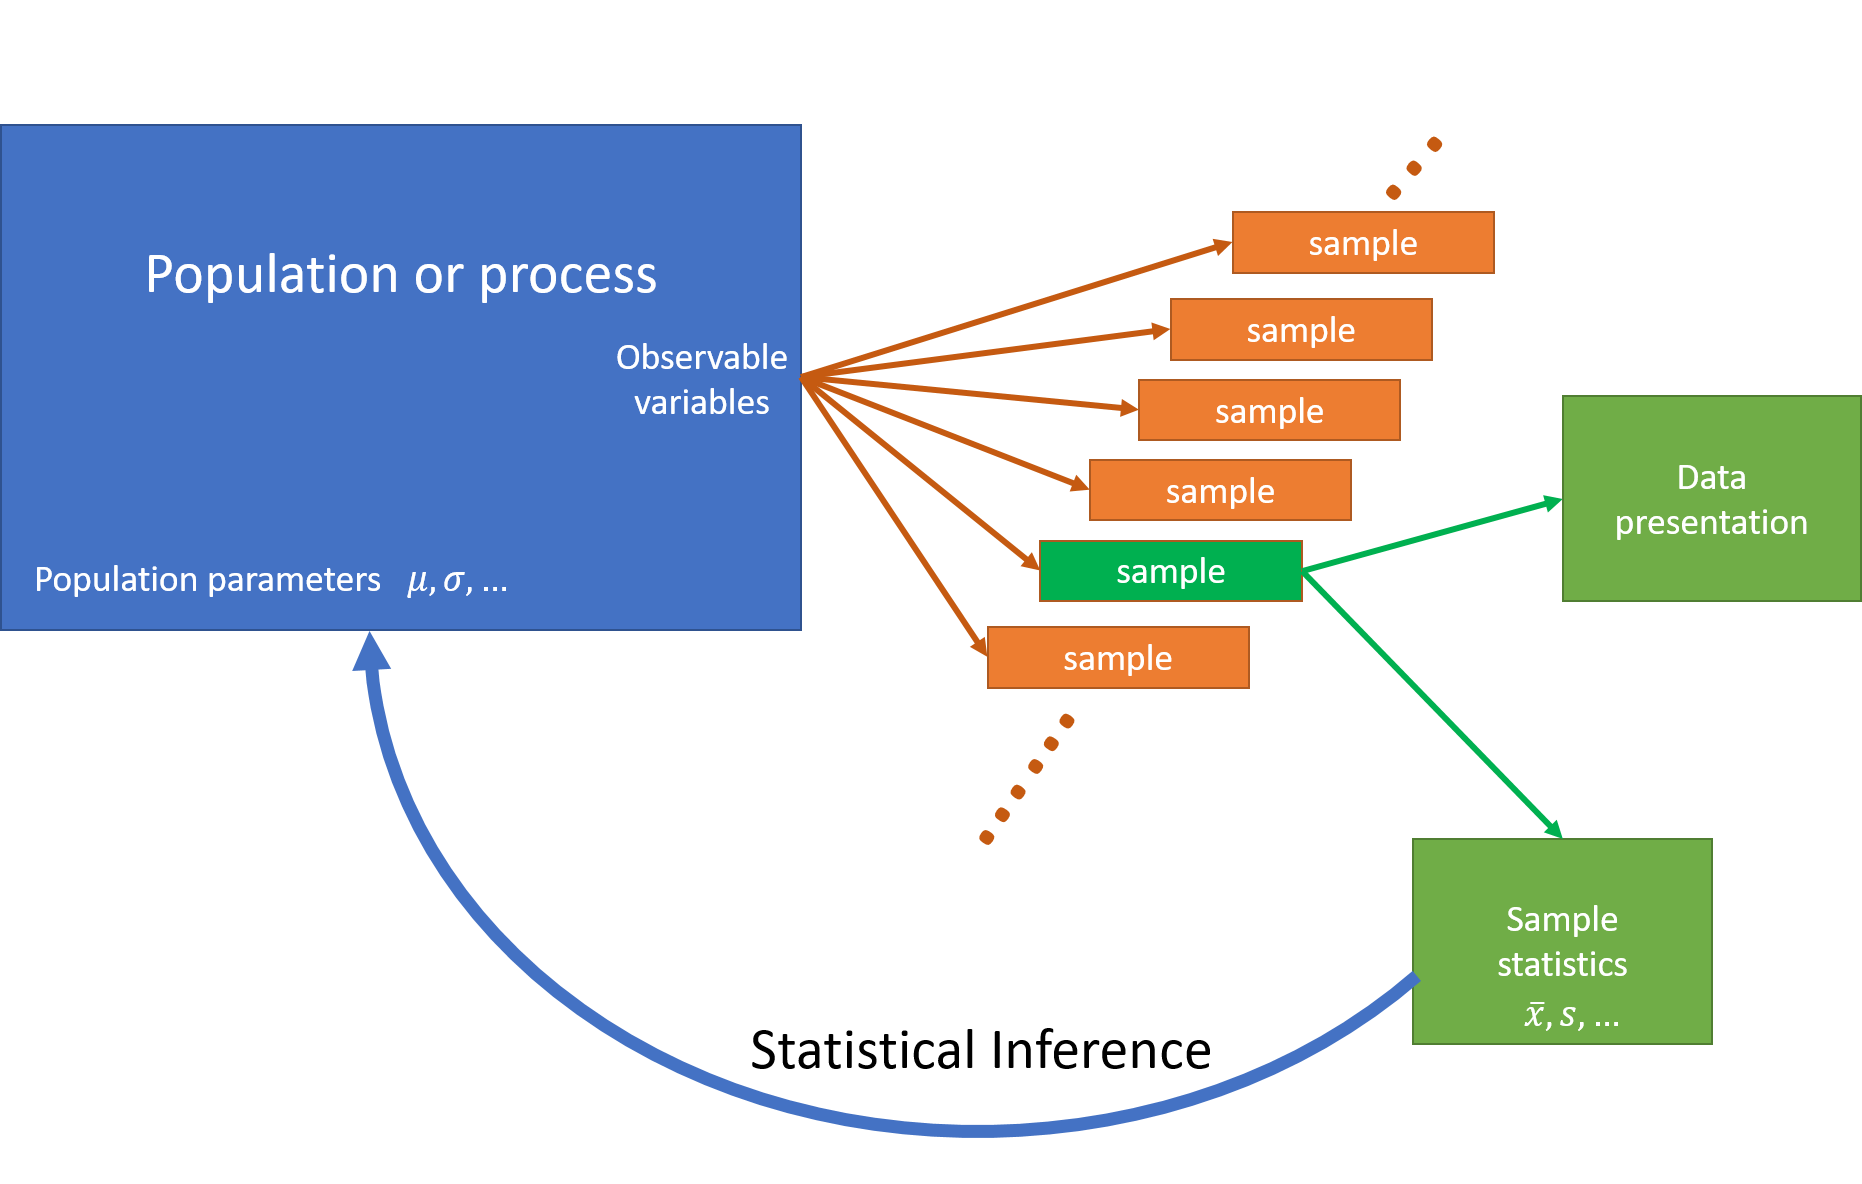
\includegraphics[width=1\linewidth]{include-files/fig/StatisticalInference} 

}

\caption{Statistical Inference}\label{fig:statistical-infrence}
\end{figure}

(One exception is when we do a \textbf{census} where we select and get fully accurate data
from every member of the population. Then there's no uncertainty left at all,
and our sampling errors are zero.)

When generating \textbf{simulated} datasets we also generate samples. Simulation
is often done as a means of testing out statistical ideas and methods,
or (in the case of the bootstrap method) when conventional ways of estimating
standard errors (and therefore confidence intervals) don't work.

Before we get into detail of estimation and inference, let's spend some time
thinking about how sampling works.

\section{Random numbers}\label{random-numbers}

In both settings (sampling and simulation) we need to start with a method
of generating random numbers. We'll start by assuming we have
some means of generating a random sequence of numbers uniformly
distributed in the interval {[}0,1{]}:
\[
    U_i \sim \text{Uniform}(0,1)\qquad \text{for $i=1,2,3, \ldots$}
\]
Here `uniformly distributed' means that all values in the range {[}0,1{]} are
equally likely to occur.

In R this is done using the \texttt{runif()} function. For example to generate 5
random draws from Uniform(0,1):

\begin{Shaded}
\begin{Highlighting}[]
\FunctionTok{runif}\NormalTok{(}\DecValTok{5}\NormalTok{)}
\end{Highlighting}
\end{Shaded}

\begin{verbatim}
## [1] 0.2875775 0.7883051 0.4089769 0.8830174 0.9404673
\end{verbatim}

Another draw will a different set of random numbers:

\begin{Shaded}
\begin{Highlighting}[]
\FunctionTok{runif}\NormalTok{(}\DecValTok{5}\NormalTok{)}
\end{Highlighting}
\end{Shaded}

\begin{verbatim}
## [1] 0.0455565 0.5281055 0.8924190 0.5514350 0.4566147
\end{verbatim}

If we draw a histogram of 100 draws it looks a bit lumpy:

\begin{Shaded}
\begin{Highlighting}[]
\FunctionTok{hist}\NormalTok{(}\FunctionTok{runif}\NormalTok{(}\DecValTok{100}\NormalTok{), }\AttributeTok{xlab=}\StringTok{"x"}\NormalTok{, }\AttributeTok{ylab=}\StringTok{"Frequency"}\NormalTok{)}
\end{Highlighting}
\end{Shaded}

\begin{figure}

{\centering 
\includegraphics{_main_files/figure-latex/unnamed-chunk-7-1} 

}

\caption{100 draws from Uniform(0,1)}\label{fig:unnamed-chunk-7}
\end{figure}

But a histogram of 100,000 draws is very uniform:

\begin{Shaded}
\begin{Highlighting}[]
\FunctionTok{hist}\NormalTok{(}\FunctionTok{runif}\NormalTok{(}\DecValTok{100000}\NormalTok{), }\AttributeTok{xlab=}\StringTok{"x"}\NormalTok{, }\AttributeTok{ylab=}\StringTok{"Frequency"}\NormalTok{)}
\end{Highlighting}
\end{Shaded}

\begin{figure}

{\centering 
\includegraphics{_main_files/figure-latex/unnamed-chunk-8-1} 

}

\caption{100000 draws from Uniform(0,1)}\label{fig:unnamed-chunk-8}
\end{figure}

Although the numbers appear to be random they are in fact generated using
formulae, so if one knows the formula the sequence of random numbers generated by
\texttt{runif()} is completed predictable. However the formula
is complex enough that there are no easily discernible patterns in sequences of
many millions of draws. These numbers are \textbf{psuedo-random}, but they are
random enough for our purposes.

Underlying the random number generator is a \textbf{seed} value, which initiates the
sequence. If we set the seed to a particular value, the sequence of random
numbers that will be generated after doing so will always be the same.

\begin{Shaded}
\begin{Highlighting}[]
\FunctionTok{set.seed}\NormalTok{(}\DecValTok{111}\NormalTok{)}
\FunctionTok{runif}\NormalTok{(}\DecValTok{5}\NormalTok{)}
\end{Highlighting}
\end{Shaded}

\begin{verbatim}
## [1] 0.5929813 0.7264811 0.3704220 0.5149238 0.3776632
\end{verbatim}

\begin{Shaded}
\begin{Highlighting}[]
\FunctionTok{runif}\NormalTok{(}\DecValTok{5}\NormalTok{)}
\end{Highlighting}
\end{Shaded}

\begin{verbatim}
## [1] 0.41833733 0.01065785 0.53229524 0.43216062 0.09368152
\end{verbatim}

\begin{Shaded}
\begin{Highlighting}[]
\FunctionTok{runif}\NormalTok{(}\DecValTok{5}\NormalTok{)}
\end{Highlighting}
\end{Shaded}

\begin{verbatim}
## [1] 0.55577991 0.59022849 0.06714114 0.04754785 0.15620252
\end{verbatim}

\begin{Shaded}
\begin{Highlighting}[]
\FunctionTok{set.seed}\NormalTok{(}\DecValTok{8}\NormalTok{)}
\FunctionTok{runif}\NormalTok{(}\DecValTok{5}\NormalTok{)}
\end{Highlighting}
\end{Shaded}

\begin{verbatim}
## [1] 0.4662952 0.2078233 0.7996580 0.6518713 0.3215092
\end{verbatim}

\begin{Shaded}
\begin{Highlighting}[]
\FunctionTok{set.seed}\NormalTok{(}\DecValTok{111}\NormalTok{)}
\FunctionTok{runif}\NormalTok{(}\DecValTok{5}\NormalTok{)}
\end{Highlighting}
\end{Shaded}

\begin{verbatim}
## [1] 0.5929813 0.7264811 0.3704220 0.5149238 0.3776632
\end{verbatim}

This property can be very useful when testing and comparing algorithms:
we can generate an identical sequence of random numbers and check (for
example) that two methods of estimation give the same results on
two identical randomly generated datasets.

\section{Sampling from categorical random variables}\label{sampling-from-categorical-random-variables}

Draws from a uniform distribution are all we need to simulate/sample
from any distribution.

\textbf{Heads or tails}: if the probability of flipping heads is 0.5,
we can generate \texttt{n} random numbers, and then label any values less
than 0.5 as Heads and the remainder as tails.

\begin{Shaded}
\begin{Highlighting}[]
\NormalTok{n }\OtherTok{\textless{}{-}} \DecValTok{10}
\NormalTok{u }\OtherTok{\textless{}{-}} \FunctionTok{runif}\NormalTok{(n)}
\NormalTok{u}
\end{Highlighting}
\end{Shaded}

\begin{verbatim}
##  [1] 0.2875775 0.7883051 0.4089769 0.8830174 0.9404673 0.0455565 0.5281055
##  [8] 0.8924190 0.5514350 0.4566147
\end{verbatim}

\begin{Shaded}
\begin{Highlighting}[]
\NormalTok{y }\OtherTok{\textless{}{-}} \FunctionTok{ifelse}\NormalTok{(u}\SpecialCharTok{\textless{}=}\FloatTok{0.5}\NormalTok{,}\StringTok{"Heads"}\NormalTok{,}\StringTok{"Tails"}\NormalTok{)}
\NormalTok{y}
\end{Highlighting}
\end{Shaded}

\begin{verbatim}
##  [1] "Heads" "Tails" "Heads" "Tails" "Tails" "Heads" "Tails" "Tails" "Tails"
## [10] "Heads"
\end{verbatim}

\begin{Shaded}
\begin{Highlighting}[]
\FunctionTok{table}\NormalTok{(y)}
\end{Highlighting}
\end{Shaded}

\begin{verbatim}
## y
## Heads Tails 
##     4     6
\end{verbatim}

\begin{Shaded}
\begin{Highlighting}[]
\FunctionTok{table}\NormalTok{(}\FunctionTok{ifelse}\NormalTok{(}\FunctionTok{runif}\NormalTok{(}\DecValTok{10000}\NormalTok{)}\SpecialCharTok{\textless{}=}\FloatTok{0.5}\NormalTok{,}\StringTok{"Heads"}\NormalTok{,}\StringTok{"Tails"}\NormalTok{))}
\end{Highlighting}
\end{Shaded}

\begin{verbatim}
## 
## Heads Tails 
##  5059  4941
\end{verbatim}

We can extend this idea to any set of categories.

\textbf{Red, Green or Blue}: Say we have a six sided die: three sides are red, two are green and one is blue.
The probabilities of rolling the three colours are therefore \(\frac12\), \(\frac13\), \(\frac16\) respectively.\\
These probabilities add to one.

The random variable \(Y\) is the colour that the die shows when we roll it.

\begin{Shaded}
\begin{Highlighting}[]
\NormalTok{pp }\OtherTok{\textless{}{-}} \FunctionTok{c}\NormalTok{(}\AttributeTok{Red=}\DecValTok{1}\SpecialCharTok{/}\DecValTok{2}\NormalTok{, }\AttributeTok{Green=}\DecValTok{1}\SpecialCharTok{/}\DecValTok{3}\NormalTok{, }\AttributeTok{Blue=}\DecValTok{1}\SpecialCharTok{/}\DecValTok{6}\NormalTok{)}
\FunctionTok{sum}\NormalTok{(pp)}
\end{Highlighting}
\end{Shaded}

\begin{verbatim}
## [1] 1
\end{verbatim}

In general we might have \(m\) categories, where the probability of that \(Y\)
category \(k\) is \(p_k\): \(\Pr(Y=k)=p_k\). and
\[
   \sum_{k=1}^m p_k = 1
\]
We then compute the \textbf{cumulative probabilities} \(c_k\), the partial sums of these probabilities:
\[
   c_k = \sum_{j=1}^k p_j
\]
The final cumulative probability \(c_m\) is always 1 by definition.

Implicitly we also have a value \(c_0=0\), which is the the empty sum and always
equal to zero.

These cumulative probabilities \(c_k\) are 'the probability that random variable \(Y\) has
a category label less than or equal to \(k\):
\[
    \Pr(Y\leq k) = c_k = \sum_{j=1}^k p_j
\]

\textbf{Red, Green or Blue}: the cumulative probabilities are
\begin{eqnarray*}
  c_0 &=& 0.0000\\
  c_1 &=& p_1 = 0.5000\\
  c_2 &=& p_1+p_2 = 0.5000 + 0.3333 = 0.8333\\
  c_3 &=& p_1+p_2+p_3 = 0.5000 + 0.3333 + 0.1667 = 1.0000
\end{eqnarray*}

\begin{Shaded}
\begin{Highlighting}[]
\NormalTok{m }\OtherTok{\textless{}{-}} \FunctionTok{length}\NormalTok{(pp) }\CommentTok{\# Number of categories}
\NormalTok{cp }\OtherTok{\textless{}{-}} \FunctionTok{cumsum}\NormalTok{(pp)}
\NormalTok{cp}
\end{Highlighting}
\end{Shaded}

\begin{verbatim}
##       Red     Green      Blue 
## 0.5000000 0.8333333 1.0000000
\end{verbatim}

We then take a set of uniform random numbers \(u_1,\ldots,u_n\). We then
want to find which of the \(m\) labels corresponds to each random number \(u_i\).

The rule is that if \(u_i\) is less than cumulative probability \(c_k\) but
greater than \(c_{k-1}\), then we assign the label \(k\).

There are various ways to do this, here's a version using \texttt{case\_when()} from
the \texttt{dplyr} package:

\begin{Shaded}
\begin{Highlighting}[]
\FunctionTok{set.seed}\NormalTok{(}\DecValTok{112}\NormalTok{)}
\NormalTok{u }\OtherTok{\textless{}{-}} \FunctionTok{runif}\NormalTok{(}\DecValTok{8}\NormalTok{)}
\NormalTok{u}
\end{Highlighting}
\end{Shaded}

\begin{verbatim}
## [1] 0.37667253 0.92201944 0.99187774 0.97723602 0.23629728 0.10706678 0.03915213
## [8] 0.72802690
\end{verbatim}

\begin{Shaded}
\begin{Highlighting}[]
\NormalTok{y }\OtherTok{\textless{}{-}} \FunctionTok{case\_when}\NormalTok{(u }\SpecialCharTok{\textless{}=}\NormalTok{ cp[}\DecValTok{1}\NormalTok{] }\SpecialCharTok{\textasciitilde{}} \StringTok{"Red"}\NormalTok{,}
\NormalTok{               u }\SpecialCharTok{\textless{}=}\NormalTok{ cp[}\DecValTok{2}\NormalTok{] }\SpecialCharTok{\textasciitilde{}} \StringTok{"Green"}\NormalTok{,}
               \AttributeTok{.default=}\StringTok{"Blue"}\NormalTok{)   }\CommentTok{\# here .default means "otherwise"}
\FunctionTok{data.frame}\NormalTok{(}\FunctionTok{round}\NormalTok{(u,}\DecValTok{5}\NormalTok{),y)}
\end{Highlighting}
\end{Shaded}

\begin{verbatim}
##   round.u..5.     y
## 1     0.37667   Red
## 2     0.92202  Blue
## 3     0.99188  Blue
## 4     0.97724  Blue
## 5     0.23630   Red
## 6     0.10707   Red
## 7     0.03915   Red
## 8     0.72803 Green
\end{verbatim}

\begin{Shaded}
\begin{Highlighting}[]
\FunctionTok{table}\NormalTok{(y)}
\end{Highlighting}
\end{Shaded}

\begin{verbatim}
## y
##  Blue Green   Red 
##     3     1     4
\end{verbatim}

\begin{Shaded}
\begin{Highlighting}[]
\FunctionTok{table}\NormalTok{(y)}\SpecialCharTok{/}\FunctionTok{length}\NormalTok{(y)}
\end{Highlighting}
\end{Shaded}

\begin{verbatim}
## y
##  Blue Green   Red 
## 0.375 0.125 0.500
\end{verbatim}

Note that the categories in the table haven't come out in the Red-Green-Blue order that we want -
instead they're in the default alphabetical order.

We can fix this by converting \texttt{y} to a \texttt{factor} object:

\begin{Shaded}
\begin{Highlighting}[]
\NormalTok{y }\OtherTok{\textless{}{-}} \FunctionTok{factor}\NormalTok{(y,}\AttributeTok{levels=}\FunctionTok{names}\NormalTok{(pp))}
\FunctionTok{table}\NormalTok{(y)}
\end{Highlighting}
\end{Shaded}

\begin{verbatim}
## y
##   Red Green  Blue 
##     4     1     3
\end{verbatim}

Here's what is really going on: we if we plot the cumulative probabilities as
a staircase -- a \textbf{cumulative distribution function (CDF)} then
we draw \(u_i\) from a Uniform(0,1) distribution, and then find where
a horizontal line drawn at the level of \(u_i\) intersects the CDF: and that
is the value of the categorical variable \(y_i\).

The larger the probability \(p_k\) the bigger the jump in the staircase, and
the larger the probability that category \(k\) will be selected.

\begin{figure}

{\centering 
\includegraphics{_main_files/figure-latex/unnamed-chunk-19-1} 

}

\caption{Drawing a random category}\label{fig:unnamed-chunk-19}
\end{figure}

\begin{figure}

{\centering 
\includegraphics{_main_files/figure-latex/unnamed-chunk-20-1} 

}

\caption{Drawing a random category}\label{fig:unnamed-chunk-20}
\end{figure}

\begin{Shaded}
\begin{Highlighting}[]
\FunctionTok{set.seed}\NormalTok{(}\DecValTok{112}\NormalTok{)}
\NormalTok{n }\OtherTok{\textless{}{-}} \DecValTok{10000}
\NormalTok{u }\OtherTok{\textless{}{-}} \FunctionTok{runif}\NormalTok{(n)}
\NormalTok{y }\OtherTok{\textless{}{-}} \FunctionTok{case\_when}\NormalTok{(u }\SpecialCharTok{\textless{}=}\NormalTok{ cp[}\DecValTok{1}\NormalTok{] }\SpecialCharTok{\textasciitilde{}} \StringTok{"Red"}\NormalTok{,}
\NormalTok{               u }\SpecialCharTok{\textless{}=}\NormalTok{ cp[}\DecValTok{2}\NormalTok{] }\SpecialCharTok{\textasciitilde{}} \StringTok{"Green"}\NormalTok{,}
               \AttributeTok{.default=}\StringTok{"Blue"}\NormalTok{)}
\NormalTok{y }\OtherTok{\textless{}{-}} \FunctionTok{factor}\NormalTok{(y, }\AttributeTok{levels=}\FunctionTok{names}\NormalTok{(pp))}
\FunctionTok{table}\NormalTok{(y)}
\end{Highlighting}
\end{Shaded}

\begin{verbatim}
## y
##   Red Green  Blue 
##  4976  3336  1688
\end{verbatim}

The \texttt{sample()} function implements this conveniently: select from the integers
1 to \texttt{m}

\begin{Shaded}
\begin{Highlighting}[]
\NormalTok{n }\OtherTok{\textless{}{-}} \DecValTok{10000}
\NormalTok{y }\OtherTok{\textless{}{-}} \FunctionTok{sample}\NormalTok{(m, }\AttributeTok{size=}\NormalTok{n, }\AttributeTok{prob=}\NormalTok{pp, }\AttributeTok{replace=}\ConstantTok{TRUE}\NormalTok{)}
\FunctionTok{table}\NormalTok{(y)}
\end{Highlighting}
\end{Shaded}

\begin{verbatim}
## y
##    1    2    3 
## 5014 3350 1636
\end{verbatim}

(need \texttt{replace=TRUE} here, see below).

\ldots{} or state the vector \texttt{1:m} explicitly

\begin{Shaded}
\begin{Highlighting}[]
\NormalTok{y }\OtherTok{\textless{}{-}} \FunctionTok{sample}\NormalTok{(}\DecValTok{1}\SpecialCharTok{:}\NormalTok{m, }\AttributeTok{size=}\NormalTok{n, }\AttributeTok{prob=}\NormalTok{pp, }\AttributeTok{replace=}\ConstantTok{TRUE}\NormalTok{)}
\FunctionTok{table}\NormalTok{(y)}
\end{Highlighting}
\end{Shaded}

\begin{verbatim}
## y
##    1    2    3 
## 5010 3371 1619
\end{verbatim}

\ldots{} or directly from the vector of labels \ldots{}

\begin{Shaded}
\begin{Highlighting}[]
\NormalTok{y }\OtherTok{\textless{}{-}} \FunctionTok{sample}\NormalTok{(}\FunctionTok{c}\NormalTok{(}\StringTok{"Red"}\NormalTok{,}\StringTok{"Green"}\NormalTok{,}\StringTok{"Blue"}\NormalTok{), }\AttributeTok{size=}\NormalTok{n, }\AttributeTok{prob=}\NormalTok{pp, }\AttributeTok{replace=}\ConstantTok{TRUE}\NormalTok{)}
\NormalTok{y }\OtherTok{\textless{}{-}} \FunctionTok{factor}\NormalTok{(y,}\AttributeTok{levels=}\FunctionTok{names}\NormalTok{(pp))}
\FunctionTok{table}\NormalTok{(y)}
\end{Highlighting}
\end{Shaded}

\begin{verbatim}
## y
##   Red Green  Blue 
##  4980  3325  1695
\end{verbatim}

\ldots{} get the labels from \texttt{pp} \ldots{}

\begin{Shaded}
\begin{Highlighting}[]
\NormalTok{y }\OtherTok{\textless{}{-}} \FunctionTok{sample}\NormalTok{(}\FunctionTok{names}\NormalTok{(pp), }\AttributeTok{size=}\NormalTok{n, }\AttributeTok{prob=}\NormalTok{pp, }\AttributeTok{replace=}\ConstantTok{TRUE}\NormalTok{)}
\NormalTok{y }\OtherTok{\textless{}{-}} \FunctionTok{factor}\NormalTok{(y,}\AttributeTok{levels=}\FunctionTok{names}\NormalTok{(pp))}
\FunctionTok{table}\NormalTok{(y)}
\end{Highlighting}
\end{Shaded}

\begin{verbatim}
## y
##   Red Green  Blue 
##  4994  3389  1617
\end{verbatim}

\section{Sampling from discrete numerical random variables}\label{sampling-from-discrete-numerical-random-variables}

The ideas above carry straight over to discrete numerical random variables.

The Binomial distribution \(Y\sim\text{Bin}(m,p)\) is the number
of successes in \(m\) trials where the probability of success on each
trial is the same \(p\), and all the trials are independent.

\(Y\) takes values 0 to \(m\), and those probabilities can be calculated by
\[
   P(Y=k) = \binom{m}{k} p^k (1-p)^{m-k} = \frac{m!}{k!(m-k)!} p^k (1-p)^{m-k}
\]
R provides these probabilities in the function \texttt{dbinom()}

e.g.~\(m=10\) rolls of a six-sided die, and \(Y\) is the number of times we get a 1,
so \(p=1/6\)

\begin{Shaded}
\begin{Highlighting}[]
\NormalTok{m }\OtherTok{\textless{}{-}} \DecValTok{10}
\NormalTok{p }\OtherTok{\textless{}{-}} \DecValTok{1}\SpecialCharTok{/}\DecValTok{6}
\NormalTok{pp }\OtherTok{\textless{}{-}} \FunctionTok{dbinom}\NormalTok{(}\DecValTok{0}\SpecialCharTok{:}\NormalTok{m, m, p)}
\NormalTok{pp}
\end{Highlighting}
\end{Shaded}

\begin{verbatim}
##  [1] 1.615056e-01 3.230112e-01 2.907100e-01 1.550454e-01 5.426588e-02
##  [6] 1.302381e-02 2.170635e-03 2.480726e-04 1.860544e-05 8.269086e-07
## [11] 1.653817e-08
\end{verbatim}

\begin{Shaded}
\begin{Highlighting}[]
\FunctionTok{barplot}\NormalTok{(pp, }\AttributeTok{names=}\DecValTok{0}\SpecialCharTok{:}\NormalTok{m,}
        \AttributeTok{xlab=}\StringTok{"y"}\NormalTok{, }\AttributeTok{ylab=}\StringTok{"Pr(Y=y)"}\NormalTok{,}
        \AttributeTok{main=}\FunctionTok{bquote}\NormalTok{(}\StringTok{"Bin("}\SpecialCharTok{*}\NormalTok{.(m)}\SpecialCharTok{*}\StringTok{","}\SpecialCharTok{*}\NormalTok{.(}\FunctionTok{sprintf}\NormalTok{(}\StringTok{" \%.4f"}\NormalTok{,p))}\SpecialCharTok{*}\StringTok{")"}\NormalTok{))}
\end{Highlighting}
\end{Shaded}

\begin{figure}

{\centering 
\includegraphics{_main_files/figure-latex/unnamed-chunk-27-1} 

}

\caption{Binomial probabilities}\label{fig:unnamed-chunk-27}
\end{figure}

The CDF is given by the function \texttt{pbinom()}

\begin{Shaded}
\begin{Highlighting}[]
\NormalTok{cp }\OtherTok{\textless{}{-}} \FunctionTok{pbinom}\NormalTok{(}\DecValTok{0}\SpecialCharTok{:}\NormalTok{m, m, p)}
\end{Highlighting}
\end{Shaded}

\begin{Shaded}
\begin{Highlighting}[]
\FunctionTok{plot}\NormalTok{(}\DecValTok{0}\SpecialCharTok{:}\NormalTok{m, cp, }\AttributeTok{type=}\StringTok{"s"}\NormalTok{,}
        \AttributeTok{xlab=}\StringTok{"y"}\NormalTok{, }\AttributeTok{ylab=}\StringTok{"Pr(Y\textless{}=y)"}\NormalTok{,}
        \AttributeTok{main=}\FunctionTok{bquote}\NormalTok{(}\StringTok{"Bin("}\SpecialCharTok{*}\NormalTok{.(m)}\SpecialCharTok{*}\StringTok{","}\SpecialCharTok{*}\NormalTok{.(}\FunctionTok{sprintf}\NormalTok{(}\StringTok{" \%.4f"}\NormalTok{,p))}\SpecialCharTok{*}\StringTok{")"}\NormalTok{))}
\end{Highlighting}
\end{Shaded}

\begin{figure}

{\centering 
\includegraphics{_main_files/figure-latex/unnamed-chunk-29-1} 

}

\caption{Binomial CDF}\label{fig:unnamed-chunk-29}
\end{figure}

Drawing a single value of \(Y\) proceeds the same way as for a categorical
variable:

\begin{figure}

{\centering 
\includegraphics{_main_files/figure-latex/unnamed-chunk-30-1} 

}

\caption{Drawing from a Binomial(10,1/6) distribution}\label{fig:unnamed-chunk-30}
\end{figure}

So we can draw multiple values of \(Y\) from Bin(10,\(\frac16\))
using the \texttt{sample()} function:

\begin{Shaded}
\begin{Highlighting}[]
\NormalTok{n }\OtherTok{\textless{}{-}} \DecValTok{10000}
\NormalTok{pp }\OtherTok{\textless{}{-}} \FunctionTok{dbinom}\NormalTok{(}\DecValTok{0}\SpecialCharTok{:}\NormalTok{m, m, p)}
\NormalTok{y }\OtherTok{\textless{}{-}} \FunctionTok{sample}\NormalTok{(}\DecValTok{0}\SpecialCharTok{:}\NormalTok{m, n, }\AttributeTok{prob=}\NormalTok{pp, }\AttributeTok{replace=}\ConstantTok{TRUE}\NormalTok{)}
\FunctionTok{barplot}\NormalTok{(}\FunctionTok{table}\NormalTok{(y))}
\end{Highlighting}
\end{Shaded}

\begin{figure}

{\centering 
\includegraphics{_main_files/figure-latex/unnamed-chunk-31-1} 

}

\caption{10000 draws from a Binomial(10,1/6)}\label{fig:unnamed-chunk-31}
\end{figure}

Of course R provides a specific function for doing the same thing: \texttt{rbinom()}

\begin{Shaded}
\begin{Highlighting}[]
\NormalTok{n }\OtherTok{\textless{}{-}} \DecValTok{10000}
\NormalTok{y }\OtherTok{\textless{}{-}} \FunctionTok{rbinom}\NormalTok{(n, m, p)}
\FunctionTok{barplot}\NormalTok{(}\FunctionTok{table}\NormalTok{(y))}
\end{Highlighting}
\end{Shaded}

\begin{figure}

{\centering 
\includegraphics{_main_files/figure-latex/unnamed-chunk-32-1} 

}

\caption{10000 draws from a Binomial(10,1/6)}\label{fig:unnamed-chunk-32}
\end{figure}

But that function is just doing what we've described above using \texttt{sample()}.

A particular common example is where we have \(m\) objects and want to select
one of them at random, with each object having equal probability of being
selected: i.e.~each has probability \(1/m\).

\section{Sampling from continuous random variables}\label{sampling-from-continuous-random-variables}

Continous random variables are simulated using the same principle.

The cumulative distribution function (CDF) of a continuous random variable \(Y\) is
defined to be
\[
   F(y) = \Pr(Y\leq y) = \int_{-\infty}^y f(y')\;{\rm d}y'
\]

\begin{figure}

{\centering 
\includegraphics{_main_files/figure-latex/unnamed-chunk-33-1} 

}

\caption{Normal distribution density and CDF}\label{fig:unnamed-chunk-33}
\end{figure}

We can use \(F(y)\) to draw a random value from the distribution of \(Y\)
by first drawing a random value \(U\) from a Uniform(0,1) distribution.

We then solve the equation
\[
   U = F(y)
\]
for \(y\): i.e.~find the value of \(y\) corresponding to a CDF value of \(U\).

For many standard distributions (including the Normal and Gamma distributions)
there is no analytic formula which gives the solution for \(y\) given \(u\):
but there are numerical approximations which can be used in those settings.

One simple case which does have an analytic solution is the Exponential
distribution \(Y\sim\text{Exp}(\lambda)\). This is a one parameter distribution
where \(Y\) is non-negative (\(Y\geq 0\)), and can be used to model cases such
the length of time it takes for an event to occur (e.g.~the length of time for a
radioactive nucleus to decay). The single parameter \(\lambda\) is the \textbf{rate}
(e.g.~number of radioactive decay events per unit time).

The exponential distribution has probability density function
\[
   f(y) = \lambda e^{-\lambda y}\qquad \text{where $y\geq 0$}
\]
and has mean \(E[Y]=1/\lambda\).

\begin{figure}

{\centering 
\includegraphics{_main_files/figure-latex/unnamed-chunk-34-1} 

}

\caption{Exponential probability distribution}\label{fig:unnamed-chunk-34}
\end{figure}

The CDF is the integral of the probability density function
\[
   \Pr(Y\leq y) = F(y) = \int_0^y f(y)\,{\rm d}y
\]
which for the Exponential distribution is
\[
  F(y) = \int_0^y \lambda e^{-\lambda t} {\rm d}t = 1 - e^{-\lambda y}
\]

\begin{figure}

{\centering 
\includegraphics{_main_files/figure-latex/unnamed-chunk-35-1} 

}

\caption{Exponential cumulative probability distribution}\label{fig:unnamed-chunk-35}
\end{figure}

Solving
\[
   u = F(y) = 1-e^{-\lambda y}
\]
for \(y\) leads to
\[
   y = -\frac{1}{\lambda}\log(1-u)
\]

Using this function we can easily draw directly from an
Exponential distribution.

\begin{Shaded}
\begin{Highlighting}[]
\NormalTok{n }\OtherTok{\textless{}{-}} \DecValTok{10000}
\NormalTok{u }\OtherTok{\textless{}{-}} \FunctionTok{runif}\NormalTok{(n)}
\NormalTok{lambda }\OtherTok{\textless{}{-}} \FloatTok{0.5}
\NormalTok{y }\OtherTok{\textless{}{-}} \SpecialCharTok{{-}}\NormalTok{(}\DecValTok{1}\SpecialCharTok{/}\NormalTok{lambda)}\SpecialCharTok{*}\FunctionTok{log}\NormalTok{(}\DecValTok{1}\SpecialCharTok{{-}}\NormalTok{u)}
\FunctionTok{mean}\NormalTok{(y)}
\end{Highlighting}
\end{Shaded}

\begin{verbatim}
## [1] 1.990456
\end{verbatim}

\begin{Shaded}
\begin{Highlighting}[]
\FunctionTok{hist}\NormalTok{(y, }\AttributeTok{main=}\StringTok{"Histogram of draws from Exp(0.5)"}\NormalTok{)}
\end{Highlighting}
\end{Shaded}

\begin{figure}

{\centering 
\includegraphics{_main_files/figure-latex/unnamed-chunk-36-1} 

}

\caption{10000 draws from an Exponential distribution}\label{fig:unnamed-chunk-36}
\end{figure}

\section{Sampling from a finite collection}\label{sampling-from-a-finite-collection}

The simulations discussed so far all draw from \textbf{infinite} populations:
we can set the sample size \(n\) to any value. However it often occurs that
we have only a finite population - e.g.~when drawing a random sample
of students from a class, or households from a suburb for interview.
Then the population size \(N\) is finite.

In the general case we have a set of \(N\) \textbf{units} (i.e.~students or households)
in a population of finite size, and we want to draw a sample of \(n\) of these units.

We usually start by listing or \textbf{enumerating} the units. This list is called
a \textbf{frame} or a \textbf{sample frame}.

Consider the case where we have a small street containing
\(N=10\) houses, numbered 1-10.
We want to select 5 of these houses with equal probability. There are a number of
ways we could do this.

\subsection{Sampling without replacement}\label{sampling-without-replacement}

If the houses have equal probability then we could proceed as follows:

\begin{itemize}
\tightlist
\item
  We draw a random number from 1-10, e.g.~house number 2, and mark it as selected
\item
  We draw another random number from 1-10, e.g.~house number 5, and mark it as selected
\item
  We repeat this process, but if we choose a house that is already selected, we discard that
  selection;
\item
  The process continues until we have a set of 5 distinct houses.
\end{itemize}

At the start we take our frame (i.e.~list) of houses,
and initially mark them all as unselected. Then at each step where we
successfully select a previously unselected house we mark that house as selected.

\begin{Shaded}
\begin{Highlighting}[]
\NormalTok{bigN }\OtherTok{\textless{}{-}} \DecValTok{10} \CommentTok{\# population size}
\NormalTok{frame }\OtherTok{\textless{}{-}} \FunctionTok{data.frame}\NormalTok{(}\AttributeTok{house=}\DecValTok{1}\SpecialCharTok{:}\NormalTok{bigN, }\AttributeTok{selected=}\ConstantTok{FALSE}\NormalTok{)}
\NormalTok{n }\OtherTok{\textless{}{-}} \DecValTok{5}  \CommentTok{\# sample size}
\NormalTok{nselected }\OtherTok{\textless{}{-}} \DecValTok{0}
\ControlFlowTok{while}\NormalTok{(nselected }\SpecialCharTok{\textless{}}\NormalTok{ n) \{}
\NormalTok{  i }\OtherTok{\textless{}{-}} \FunctionTok{sample}\NormalTok{(bigN, }\DecValTok{1}\NormalTok{)  }\CommentTok{\# sample a single number at random from 1:bigN with equal probability}
  \ControlFlowTok{if}\NormalTok{(}\SpecialCharTok{!}\NormalTok{frame}\SpecialCharTok{$}\NormalTok{selected[i]) \{}
\NormalTok{    frame}\SpecialCharTok{$}\NormalTok{selected[i] }\OtherTok{\textless{}{-}} \ConstantTok{TRUE}
\NormalTok{    nselected }\OtherTok{\textless{}{-}}\NormalTok{ nselected }\SpecialCharTok{+} \DecValTok{1} 
\NormalTok{  \}}
\NormalTok{\}}
\NormalTok{frame}\SpecialCharTok{$}\NormalTok{house[frame}\SpecialCharTok{$}\NormalTok{selected]}
\end{Highlighting}
\end{Shaded}

\begin{verbatim}
## [1]  1  6  7  8 10
\end{verbatim}

It's not guaranteed how many steps this process is going to take, since the number
of times we select a house that has already been selected is random. If the sample size
\(n\) is small and the population size \(N\) is large then it will take \(n\) steps, or possibly
just a few more. If \(n\) is close to \(N\) and \(N\) is large, it could take a very very
long time.

A simpler way to solve this is to assign each house a distinct random number
between 0 and 1, and then sort the frame in order of the random numbers.

\begin{Shaded}
\begin{Highlighting}[]
\NormalTok{bigN }\OtherTok{\textless{}{-}} \DecValTok{10} \CommentTok{\# population size}
\NormalTok{frame }\OtherTok{\textless{}{-}} \FunctionTok{data.frame}\NormalTok{(}\AttributeTok{house=}\DecValTok{1}\SpecialCharTok{:}\NormalTok{bigN, }\AttributeTok{selected=}\ConstantTok{FALSE}\NormalTok{)}
\NormalTok{n }\OtherTok{\textless{}{-}} \DecValTok{5}  \CommentTok{\# sample size}
\NormalTok{frame}\SpecialCharTok{$}\NormalTok{u }\OtherTok{\textless{}{-}} \FunctionTok{runif}\NormalTok{(bigN)}
\NormalTok{frame }\OtherTok{\textless{}{-}}\NormalTok{ frame[}\FunctionTok{order}\NormalTok{(frame}\SpecialCharTok{$}\NormalTok{u),]}
\NormalTok{frame}\SpecialCharTok{$}\NormalTok{selected[}\DecValTok{1}\SpecialCharTok{:}\NormalTok{n] }\OtherTok{\textless{}{-}} \ConstantTok{TRUE}
\NormalTok{frame}
\end{Highlighting}
\end{Shaded}

\begin{verbatim}
##    house selected         u
## 9      9     TRUE 0.0812427
## 4      4     TRUE 0.3739315
## 2      2     TRUE 0.4137952
## 6      6     TRUE 0.4341604
## 10    10     TRUE 0.4909159
## 3      3    FALSE 0.5850114
## 8      8    FALSE 0.8708720
## 5      5    FALSE 0.8837804
## 1      1    FALSE 0.9278206
## 7      7    FALSE 0.9475266
\end{verbatim}

\begin{Shaded}
\begin{Highlighting}[]
\NormalTok{frame }\OtherTok{\textless{}{-}}\NormalTok{ frame[}\FunctionTok{order}\NormalTok{(frame}\SpecialCharTok{$}\NormalTok{house),]}
\NormalTok{frame}\SpecialCharTok{$}\NormalTok{house[frame}\SpecialCharTok{$}\NormalTok{selected]}
\end{Highlighting}
\end{Shaded}

\begin{verbatim}
## [1]  2  4  6  9 10
\end{verbatim}

Of course, the simplest way of all is just to use the \texttt{sample()} function

\begin{Shaded}
\begin{Highlighting}[]
\NormalTok{bigN }\OtherTok{\textless{}{-}} \DecValTok{10} \CommentTok{\# population size}
\NormalTok{n }\OtherTok{\textless{}{-}} \DecValTok{5}  \CommentTok{\# sample size}
\FunctionTok{sample}\NormalTok{(bigN, n)}
\end{Highlighting}
\end{Shaded}

\begin{verbatim}
## [1] 10  4  6  3  2
\end{verbatim}

It's very often that we do have a frame, a list of objects with names, and we
want to select from this at random.

\begin{Shaded}
\begin{Highlighting}[]
\NormalTok{frame }\OtherTok{\textless{}{-}} \FunctionTok{data.frame}\NormalTok{(}\AttributeTok{Name=}\FunctionTok{c}\NormalTok{(}\StringTok{"Mark"}\NormalTok{,}\StringTok{"Chloe"}\NormalTok{,}\StringTok{"Sam"}\NormalTok{,}\StringTok{"Caitlin"}\NormalTok{,}\StringTok{"Harry"}\NormalTok{,}\StringTok{"Nina"}\NormalTok{),}
                    \AttributeTok{Age=}\FunctionTok{c}\NormalTok{(}\DecValTok{20}\NormalTok{,}\DecValTok{19}\NormalTok{,}\DecValTok{18}\NormalTok{,}\DecValTok{19}\NormalTok{,}\DecValTok{19}\NormalTok{,}\DecValTok{21}\NormalTok{),}
                    \AttributeTok{Major=}\FunctionTok{c}\NormalTok{(}\StringTok{"STAT"}\NormalTok{,}\StringTok{"STAT"}\NormalTok{,}\StringTok{"DATA"}\NormalTok{,}\StringTok{"COMP"}\NormalTok{,}\StringTok{"MATH"}\NormalTok{,}\StringTok{"STAT"}\NormalTok{))}
\NormalTok{frame}
\end{Highlighting}
\end{Shaded}

\begin{verbatim}
##      Name Age Major
## 1    Mark  20  STAT
## 2   Chloe  19  STAT
## 3     Sam  18  DATA
## 4 Caitlin  19  COMP
## 5   Harry  19  MATH
## 6    Nina  21  STAT
\end{verbatim}

We can select, say, 3 names

\begin{Shaded}
\begin{Highlighting}[]
\NormalTok{n }\OtherTok{\textless{}{-}} \DecValTok{3}
\NormalTok{samplenames }\OtherTok{\textless{}{-}} \FunctionTok{sample}\NormalTok{(frame}\SpecialCharTok{$}\NormalTok{Name, n)}
\NormalTok{samplenames}
\end{Highlighting}
\end{Shaded}

\begin{verbatim}
## [1] "Nina" "Sam"  "Mark"
\end{verbatim}

and then subset the frame

\begin{Shaded}
\begin{Highlighting}[]
\NormalTok{samplemembers }\OtherTok{\textless{}{-}}\NormalTok{ frame[frame}\SpecialCharTok{$}\NormalTok{Name}\SpecialCharTok{\%in\%}\NormalTok{samplenames,]}
\NormalTok{samplemembers}
\end{Highlighting}
\end{Shaded}

\begin{verbatim}
##   Name Age Major
## 1 Mark  20  STAT
## 3  Sam  18  DATA
## 6 Nina  21  STAT
\end{verbatim}

If you like dplyr

\begin{Shaded}
\begin{Highlighting}[]
\NormalTok{samplemembers }\OtherTok{\textless{}{-}}\NormalTok{ frame }\SpecialCharTok{\%\textgreater{}\%} 
  \FunctionTok{filter}\NormalTok{(Name}\SpecialCharTok{\%in\%}\NormalTok{samplenames)}
\NormalTok{samplemembers}
\end{Highlighting}
\end{Shaded}

\begin{verbatim}
##   Name Age Major
## 1 Mark  20  STAT
## 2  Sam  18  DATA
## 3 Nina  21  STAT
\end{verbatim}

Note we can find out where in the frame particular individuals are located

\begin{Shaded}
\begin{Highlighting}[]
\FunctionTok{match}\NormalTok{(}\FunctionTok{c}\NormalTok{(}\StringTok{\textquotesingle{}Mark\textquotesingle{}}\NormalTok{,}\StringTok{\textquotesingle{}Harry\textquotesingle{}}\NormalTok{),frame}\SpecialCharTok{$}\NormalTok{Name)}
\end{Highlighting}
\end{Shaded}

\begin{verbatim}
## [1] 1 5
\end{verbatim}

If we're sampling without replacement, note (of course) that the sample
size can be no bigger than the population size \(n\leq N\).

\subsection{Sampling with replacement}\label{sampling-with-replacement}

When selecting a sample of 5 houses it makes sense not to allow the possibility
of selecting the same house twice. So when we've selected a house we remove
it from the list of houses available to select. When using \texttt{sample()} this means
that we set \texttt{replace=FALSE}, meaning after we've selected a member of the population
we don't put it back again.

But there are occasions where we select \textbf{with replacement} is the sensible
thing to do. This means there is a chance where a unit can be selected more than
once, and this occurs in situations where we want to assign different probabilities
of selection to different units of the population.

Starting with the the case of equal probabilities, we repeatedly draw
units from the population under identical circumstances: on every draw
each unit is available for selection, and we count how many times each
unit is selected.

\begin{Shaded}
\begin{Highlighting}[]
\FunctionTok{set.seed}\NormalTok{(}\DecValTok{111}\NormalTok{)}
\NormalTok{bigN }\OtherTok{\textless{}{-}} \DecValTok{10}
\NormalTok{n }\OtherTok{\textless{}{-}} \DecValTok{5}
\FunctionTok{replicate}\NormalTok{(n, }\FunctionTok{sample}\NormalTok{(bigN, }\DecValTok{1}\NormalTok{))}
\end{Highlighting}
\end{Shaded}

\begin{verbatim}
## [1] 4 3 9 5 3
\end{verbatim}

In this sample we've drawn Unit 3 twice.

If \(n\) is small and \(bigN\) is large the probability of repeats is small. But if a repeat
happens we of course do not make our selected household repeat the questionnaire, instead
we count them twice (or as many times as they are selected) in our analysis.

Imagine our sample of 10 houses aren't actually just houses, they're farms, and some of them
are very large and some are very small. We want to give the large farms a high chance of
selection.

\begin{Shaded}
\begin{Highlighting}[]
\FunctionTok{set.seed}\NormalTok{(}\DecValTok{122}\NormalTok{)}
\NormalTok{bigN }\OtherTok{\textless{}{-}} \DecValTok{10}
\NormalTok{n }\OtherTok{\textless{}{-}} \DecValTok{5}
\NormalTok{frame }\OtherTok{\textless{}{-}} \FunctionTok{data.frame}\NormalTok{(}\AttributeTok{farm=}\DecValTok{1}\SpecialCharTok{:}\DecValTok{10}\NormalTok{, }\AttributeTok{ncows=}\FunctionTok{c}\NormalTok{(}\DecValTok{1000}\NormalTok{,}\DecValTok{5000}\NormalTok{,}\DecValTok{2000}\NormalTok{,}\DecValTok{500}\NormalTok{,}\DecValTok{500}\NormalTok{,}
                                       \DecValTok{5000}\NormalTok{,}\DecValTok{500}\NormalTok{,}\DecValTok{5000}\NormalTok{,}\DecValTok{30000}\NormalTok{,}\DecValTok{100}\NormalTok{))}
\NormalTok{frame}
\end{Highlighting}
\end{Shaded}

\begin{verbatim}
##    farm ncows
## 1     1  1000
## 2     2  5000
## 3     3  2000
## 4     4   500
## 5     5   500
## 6     6  5000
## 7     7   500
## 8     8  5000
## 9     9 30000
## 10   10   100
\end{verbatim}

\begin{Shaded}
\begin{Highlighting}[]
\FunctionTok{sample}\NormalTok{(frame}\SpecialCharTok{$}\NormalTok{farm, n, }\AttributeTok{prob=}\NormalTok{frame}\SpecialCharTok{$}\NormalTok{ncows, }\AttributeTok{replace=}\ConstantTok{TRUE}\NormalTok{)}
\end{Highlighting}
\end{Shaded}

\begin{verbatim}
## [1] 2 2 9 9 9
\end{verbatim}

Unsurprisingly, the very large farm number 9 has been selected three times here.

It \textbf{is} possible to have unequal probability sampling \textbf{without} replacement, estimation
of standard errors is complicated in such designs, so we won't be using such designs.

For now, just note that we switch to with replacement designs when we're sampling from
sets of units where want to have units with different probabilities of selection.

\chapter{Sample Surveys}\label{sample-surveys}

A sample survey is an exercise in which \textbf{data} are collected from a
\textbf{sample} (a subset) or a \textbf{population}. The data collected are used to
create \textbf{estimates} of the characteristics or \textbf{parameters} of the
population.

Some examples:

\begin{itemize}
\tightlist
\item
  A sample of voters are telephoned to ask their voting intentions, with
  the aim of predicting the outcome of the election;
\item
  A sample of sites in a river catchment is tested for the presence of
  algae to determine the spread of the algae throughout the entire catchment;
\item
  A sample of households is selected, and the residents asked about their
  employment status, in order to estimate the national unemployment rate.
\end{itemize}

A \textbf{census} is a special case of a sample survey in which every member of
the population is surveyed.

\section{The Survey Process}\label{the-survey-process}

The different steps in the survey process are shown in Figure \ref{fig:survey-process1}.

\begin{figure}

{\centering 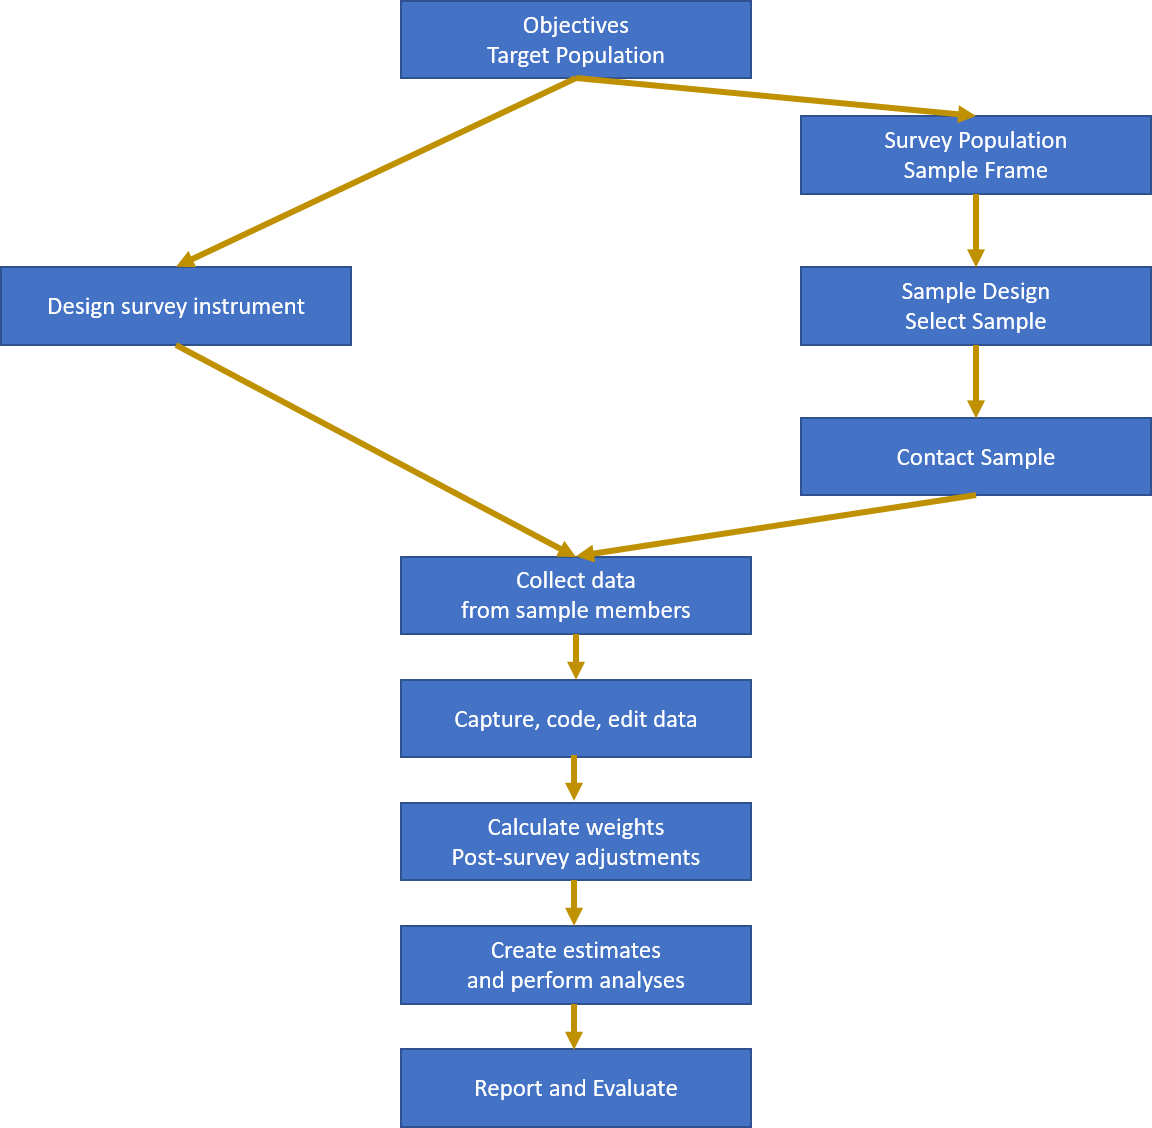
\includegraphics[width=1\linewidth]{include-files/fig/SurveyProcess1} 

}

\caption{The Survey Process}\label{fig:survey-process1}
\end{figure}

\begin{itemize}
\tightlist
\item
  Every survey has a set of \textbf{objectives} -- the particular populations
  which are of interest;
\item
  These parameters are properties of the \textbf{target population}: the
  population about which estimates are to be made;
\item
  Not all members of the target population are able to be identified: the
  ones that can be surveyed make up the \textbf{survey population};
\item
  The \textbf{sample frame} is a listing of all members of the survey
  population;
\item
  The \textbf{sample design} is the method of selecting the sample from the
  frame. The \textbf{sample size} is usually decided as a compromise between the
  required \textbf{accuracy of estimates} and the survey \textbf{costs} and other
  constraints (e.g.~the time available for the survey);
\item
  \textbf{survey instrument} is the means of data collection. It is
  usually a paper or electronic questionnaire, completed by the respondent or
  the interviewer/observer. The instrument aims to measure the properties of
  the sample members which mean that the desired population characteristic can
  be estimated. The instrument must be \textbf{valid} (it must actually measure
  what it intends to measure) and \textbf{reliable} (repeated measurements of the
  same sample member under identical circumstances should always yield similar
  results);
\item
  The sample members are \textbf{contacted} and \textbf{recruited} into the
  sample. Not all selected members will be able to be contacted (even after
  strenuous efforts), and some will not respond even if contacted;
\item
  The data are collected from the sample members in some \textbf{mode}
  (e.g.~face-to-face, telephone, web, observational, \ldots);
\item
  The data collected are \textbf{captured} (stored on a computer); \textbf{coded}
  (converted into standard classification systems); \textbf{edited} (checks for
  data consistency); and \textbf{stored} in a final dataset;
\item
  The data may be \textbf{adjusted}, e.g.~imputation or weight adjustments
  for nonresponse may be done;
\item
  \textbf{Estimates} of the parameters of interest are constructed, and other
  \textbf{analysis} of the data is carried out (e.g.~regression estimation,
  comparison with other data etc.);
\item
  The results are summarised in a \textbf{report};
\item
  The original data may be \textbf{archived} in some appropriate form,
  or \textbf{destroyed};
\item
  A post-survey \textbf{evaluation} may be made to determine how well the survey
  met its goals.
\end{itemize}

For example: The Household Labour Force Survey (HLFS).

\begin{itemize}
\tightlist
\item
  One of the main \textbf{objectives} of the HLFS is to estimate the
  unemployment rate every quarter;
\item
  The \textbf{target population} is the working age population of
  New Zealand;
\item
  The \textbf{survey population} is the civilian, non-institutionalised
  usually resident population of adults aged 15+
  living in permanent, private dwellings on the main islands of New
  Zealand (North Island, South Island and Waiheke Island);
\item
  The \textbf{sample frame} is a list of dwellings created at the most recent
  census and regularly updated to reflect changes;
\item
  The \textbf{sample design} is a stratified cluster design. Within each regional
  government area a sample of small areas (PSUs) is selected. A sample of
  households is selected from within each PSU. Every adult from the selected
  households is surveyed. 15000 households and 30000 adults are surveyed every
  three months, in order to create unemployment estimates accurate to within
  \(0.5\)\%.
\item
  The \textbf{survey instrument} is an electronic questionnaire.
\item
  The interviewers contact the households in person or by telephone,
  making up to 10 call backs to ensure contact is made. \textbf{Proxy responses}
  are permitted (i.e.~one household member can respond on behalf of another).
  The interview takes place by computer assisted personal or telephone
  interviewing (CAPI or CATI).
\item
  The results are \textbf{post-stratified} to match the current population estimates
  in each local government area;
\item
  \textbf{Estimates} of the unemployment rate are published within about 6
  weeks of the end of the quarter.
\end{itemize}

\section{Populations and Frames}\label{populations-and-frames}

The target population defines the \textbf{scope} of the survey: the set of units
which make up the population in which we are interested.

The sample frame is a method of gaining access to the members of the target
population. It is an actual or conceptual list. However it may not be
perfect (Figure \ref{fig:scope-coverage}).

\begin{itemize}
\tightlist
\item
  Not all members of the target population will appear on the sample frame:
  the missing units are \textbf{out of coverage};
\item
  Not all units listed on the sample frame are members of the target
  population: the extra units are \textbf{out of scope}.
\item
  The survey population are those units which are both in the target
  population (in scope) and on the frame (in coverage).
\end{itemize}

Our aim is to have a sample frame which covers most if not all of the target
population, and which has only very few out of scope units.

The reason for this is very important: we can make estimates about units in a population
\textbf{only} if they are included in the sample frame. This inference is possible
\textbf{whether or not we select them}. If there is a subpopulation of units that is
not on our frame (i.e.~they are out of coverage) then we can never select them, we
can never learn anything about them, and therefore we cannot make inferences about them.

\begin{figure}

{\centering 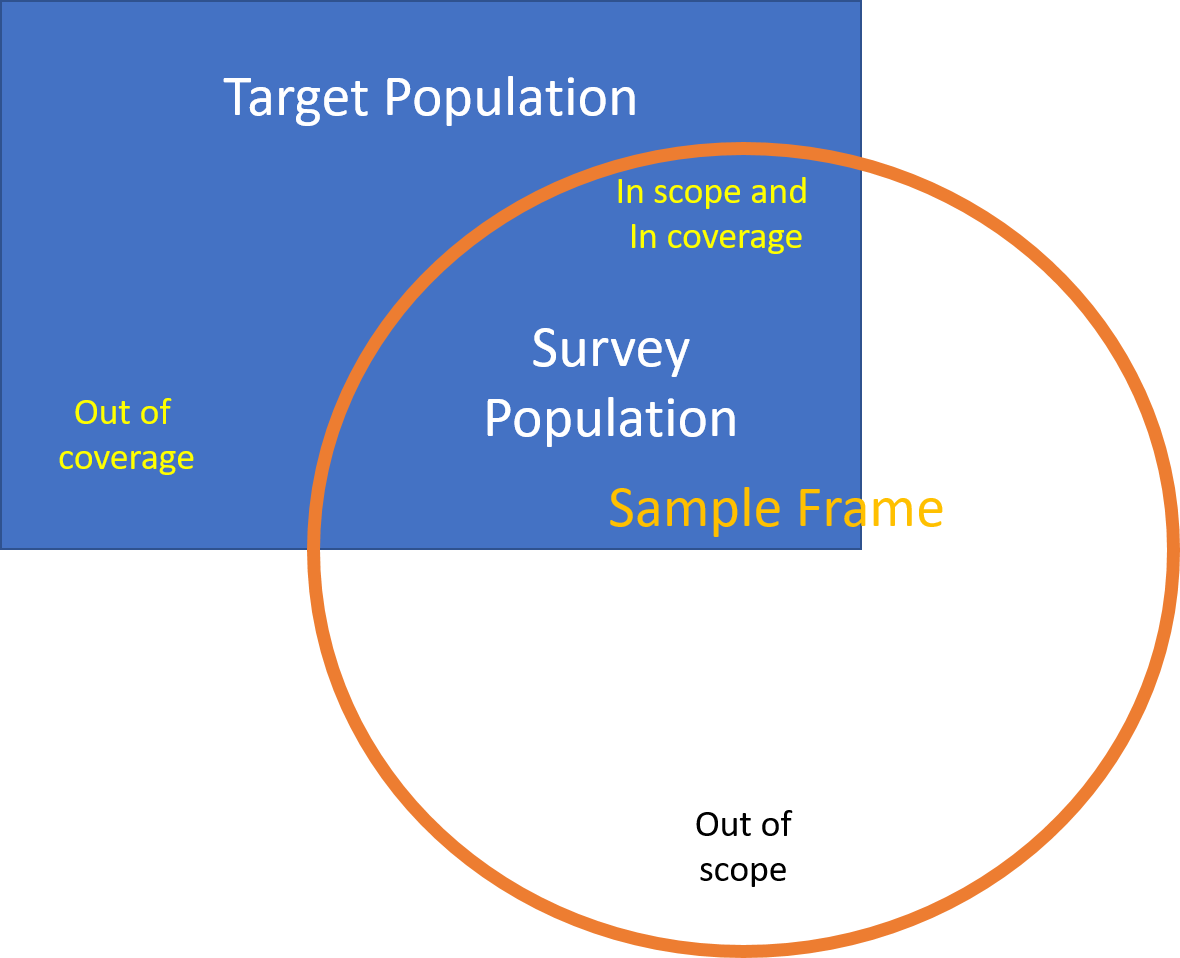
\includegraphics[width=0.7\linewidth]{include-files/fig/ScopeCoverage} 

}

\caption{Scope and Coverage}\label{fig:scope-coverage}
\end{figure}

\subsection{What is a sampling frame?}\label{what-is-a-sampling-frame}

The sampling frame is a key element in the survey process which provides the
basis from which a \emph{random} (probability based) sample can be selected. The
purpose of having a sampling frame is to enable each member of the target
population a nonzero probability of being selected to participate in the
survey. The \emph{quality} of the data, from a survey which has as its basis a
comprehensive frame, can be \emph{measured and controlled}.

The term sampling frame is sometimes misunderstood, often being thought of as a
list containing each member of the population. In fact that is more a
description of an `ideal' sampling frame. The best way to show what a sampling
frame can be in practice is to examine some examples:

\begin{itemize}
\item
  \textbf{List Frames.} Good up-to-date lists make ideal frames. However lists of
  units (electoral rolls, telephone listings etc.) are generally formed for
  purposes other than for use as sampling frames. For this reason they are
  often not close to `ideal' sampling frames. Some discussion of list frame
  problems comes later.
\item
  \textbf{Multi-stage Sampling Frames.} These frames consist of a set of lists
  which are arranged in a hierarchy of stages. For example a typical household
  survey frame will be organised like so: The first list is a a set of
  non-overlapping geographic areas from which a sample of areas is taken. For
  example we may list all the local regional councils and take a sample of
  them. Within these areas we might then list all the households and take
  samples from the household lists. From each household we would then list the
  residents and interview selections of them. Note that we do not have to list
  the entire population. The only comprehensive list needed is the list of the
  areas which will be quite small. By giving each area a chance of being
  selected we ensure each person living in each area has a chance of selection.
\item
  \textbf{Continuous Sampling Frames.} Consider the population of people entering a
  country from international flights. Suppose we choose a random number
  between one and ten (\(=k\)) and then interview the \(k\)th, \((k+10)\)th,
  \((k+20)\)th \ldots{} persons who file through customs. We will have a sample where
  every person has had a 1 in 10 chance of being selected. But what is the
  frame? There is no list. We call such a situation a `conceptual list', where
  the people filing into the country effectively formed a long queue of people
  which we have treated like a listing of the population, although a listing of
  names was never constructed. \textbackslash end\{description\}
\end{itemize}

One can find many different definitions of sampling frames. The following is a
simplified definition that should serve our purposes:

\begin{quote}
A \emph{sampling frame} is part of the system of rules and procedures used when
determining who is to be surveyed and which ensure that each member of the
population get some measurable (non-zero) chance of participating in the
survey.
\end{quote}

The examples above show that we need to think beyond the concept of a list of
units, whose construction is a separate exercise from the other survey stages.

\subsection{\texorpdfstring{What is a \emph{good} sampling frame?}{What is a good sampling frame?}}\label{what-is-a-good-sampling-frame}

We will often have several frames available and will have to decide between
different options. To help us with this decision we need to be a little more
specific about what makes a good sampling frame. The first thing we should
consider is the effective coverage of the sampling frame. This can be
determined by testing it for the following properties:

\begin{itemize}
\item
  \textbf{Each unit should be counted at least once}. If there are missing
  units (out of coverage) then the survey results may be biased if the excluded
  units tend to be different to the units which are included.
\item
  \textbf{Each unit should be counted only once}. The problem is that we
  usually can not tell how many times a unit is duplicated. This means we can
  not tell how many chances a unit has of being sampled. This can cause
  similar bias if the units which are duplicated are different to the other
  units. The results will be biased towards the duplicated sub-group of the
  population.
\item
  \textbf{Each unit should be distinguishable from the other units on the
  frame}. If we select a unit from the frame (say Jane Smith) but then can
  not tell who this refers to, when there are many Jane Smiths in the
  population, then the frame has not done its job.
\item
  \textbf{Should provide up-to-date information about the units}. For example
  it if it claims to provide Jane Smith's address it should be the current
  address.
\item
  \textbf{No units should be there if they are not meant to be}. Extra units
  (out of scope) are not a serious problem unless we fall into the elementary
  error of replacing them whenever we come across them in the sample. This
  confuses selection probabilities. The correct procedure is to drop any
  ineligible unit found in the sample and not replace them.
\item
  \textbf{Should allow direct access to each unit}. Ideally the frame will
  ultimately supply us with a list of the units we are interested in analyzing.
  Sometimes a frame will only give samples of groups of units e.g.~a list of
  addresses, each of which may contain many people. Further work is needed
  before a sample of people is realized.
\end{itemize}

\section{Approaches to sampling}\label{approaches-to-sampling}

We're talking here about random sampling, or \textbf{probability sampling}. For
the purposes of statistical inference such sampling is the only defensible method -
it's the only one that leads us to properly constructed confidence intervals
and hypothesis tests. Other approaches do exist though, and even though you'll see
them used they all have significant defects.

\begin{itemize}
\tightlist
\item
  \textbf{Probability sampling} is the gold standard: every member of the population
  has a known, non-zero chance of selection;
\item
  \textbf{Purposive sampling}: the surveyor selects members of the population that
  they consider to be representative - dangerously biased towards the views
  and prejudices of the surveyor;
\item
  \textbf{Haphazard sampling}: the surveyor uses any members of the population that
  they come across. This is what happens on the street corner when you're asked
  questions by a surveyor;
\item
  \textbf{Quota sampling}: resembles stratified sample (see later): the surveyor fills
  quotas of respondents to balance numbers of respondents in categories (e.g.~by
  age/gender/ethnicity), but does not make an accounting for non-response (see later);
\item
  \textbf{Snowball sampling}: used in rare populations that are highly connected (e.g.
  refugees from a particular country): existing sample members recruit new sample
  members using their contacts;
\item
  \textbf{Self-selected sampling}: this is the \textbf{worst} of all: the respondents themselves
  decide whether to be selected: they see an advertisement on a webpage or phone
  in with their views. Only profiles motivated population members - the silent
  majority are never measured.
\end{itemize}

\section{Example datasets}\label{example-datasets}

We'll use and re-use a number of standard datasets.

\subsection{API}\label{api}

This is a dataset on Student performance in California schools. The dataset is distributed with the \texttt{survey} library in R, and there are a number of unit record datasets which are drawn from a population dataset \texttt{apipop} under various sample designs. The population units are the schools, and a number of characteristics are available. Full documentation can be found in the \texttt{survey} package. The variables we use mostly are:

\begin{itemize}
\tightlist
\item
  \texttt{stype} - School type (Elementary/Middle/High School)
\item
  \texttt{snum} - School number
\item
  \texttt{dnum} - District number
\item
  \texttt{api99} - Academic Performance Indicator for the school in the year 1999
\item
  \texttt{api00} - Academic Performance Indicator for the school in the year 2000
\item
  \texttt{sch.wide} - Did the school meet its school-wide growth target?
\item
  \texttt{awards} - Is the school eligible for an awards program
\item
  \texttt{meals} - Percentage of students eligible for subsidised meals
\item
  \texttt{ell} - Percentage of students that are English Language Learners
\item
  \texttt{grad.sch} - Percentage of students with parents with a postgraduate education
\item
  \texttt{enroll} - Number of students enrolled
\item
  \texttt{api.stu} - Number of students tested in the API
\end{itemize}

\subsection{From the dplyr package}\label{from-the-dplyr-package}

\begin{itemize}
\tightlist
\item
  \texttt{starwars} - a list of characteristics of 87 characters from the Star Wars
  movie series;
\end{itemize}

\chapter{Statistical Inference}\label{statistical-inference}

Let's briefly review a few familiar results from earlier statistics courses.

Most of what we've done in earlier courses has assumed that we have
a \textbf{simple random sample} from an \textbf{infinite} population.

We'll use data from the \texttt{starwars} dataset (in the \texttt{dplyr} package). There
are data on 87 characters, including their heights in centimetres.\\
Six heights are missing, but let's just guess them so we have no missing data
(this process of inventing data has a respectable name: \textbf{`imputation'},
and we'll come back to it later).

\begin{Shaded}
\begin{Highlighting}[]
\FunctionTok{library}\NormalTok{(dplyr)}
\FunctionTok{data}\NormalTok{(starwars)}
\FunctionTok{sum}\NormalTok{(}\FunctionTok{is.na}\NormalTok{(starwars}\SpecialCharTok{$}\NormalTok{height))}
\end{Highlighting}
\end{Shaded}

\begin{verbatim}
## [1] 6
\end{verbatim}

\begin{Shaded}
\begin{Highlighting}[]
\NormalTok{starwars }\OtherTok{\textless{}{-}}\NormalTok{ starwars }\SpecialCharTok{\%\textgreater{}\%} 
  \FunctionTok{mutate}\NormalTok{(}\AttributeTok{height=}\FunctionTok{case\_when}\NormalTok{(name}\SpecialCharTok{==}\StringTok{"Arvel Crynyd"} \SpecialCharTok{\textasciitilde{}} \DecValTok{172}\NormalTok{, }\CommentTok{\# same as Luke}
\NormalTok{                          name}\SpecialCharTok{==}\StringTok{"Finn"} \SpecialCharTok{\textasciitilde{}} \DecValTok{172}\NormalTok{, }\CommentTok{\# same as Luke}
\NormalTok{                          name}\SpecialCharTok{==}\StringTok{"Rey"} \SpecialCharTok{\textasciitilde{}} \DecValTok{150}\NormalTok{,  }\CommentTok{\# same as Leia}
\NormalTok{                          name}\SpecialCharTok{==}\StringTok{"Poe Dameron"} \SpecialCharTok{\textasciitilde{}} \DecValTok{172}\NormalTok{, }\CommentTok{\# same as Luke}
\NormalTok{                          name}\SpecialCharTok{==}\StringTok{"BB8"} \SpecialCharTok{\textasciitilde{}} \DecValTok{96}\NormalTok{, }\CommentTok{\# same as R2D2}
\NormalTok{                          name}\SpecialCharTok{==}\StringTok{"Captain Phasma"} \SpecialCharTok{\textasciitilde{}} \DecValTok{167}\NormalTok{, }\CommentTok{\# same as C3P0}
                          \AttributeTok{.default=}\NormalTok{height))}
\end{Highlighting}
\end{Shaded}

The mean height \(\bar{Y}\) of characters in the Star Wars universe is a \textbf{population parameter}.
We can \textbf{estimate} it from a sample of characters.

\begin{quote}
\textbf{Note:} we're using capital letters for \textbf{population parameters}
(\(\bar{Y}\) is the population mean), and lower case letters for \textbf{sample statistics}
(\(\bar{y}\) is the sample mean).

It's also common to see Greek letters for \textbf{population parameters} (e.g.~\(\mu\) for the
population mean), upper case latin letters for random variables, and lower case latin letters
for sample statistics.
\end{quote}

For the purposes of this exercise let's imagine there are only \(N=87\) individuals in the entire
Star Wars universe. Let's draw a random sample of \(n=20\) from this population of \(N=87\):

\begin{Shaded}
\begin{Highlighting}[]
\FunctionTok{set.seed}\NormalTok{(}\DecValTok{222}\NormalTok{)}
\NormalTok{bigN }\OtherTok{\textless{}{-}} \FunctionTok{nrow}\NormalTok{(starwars)}
\NormalTok{n }\OtherTok{\textless{}{-}} \DecValTok{20}
\NormalTok{samplemembers }\OtherTok{\textless{}{-}}\NormalTok{ starwars[}\FunctionTok{sample}\NormalTok{(bigN, n, }\AttributeTok{replace=}\ConstantTok{FALSE}\NormalTok{),]}
\NormalTok{samplemembers }\SpecialCharTok{\%\textgreater{}\%}
\NormalTok{  dplyr}\SpecialCharTok{::}\FunctionTok{select}\NormalTok{(name,height,mass,hair\_color,homeworld) }\SpecialCharTok{\%\textgreater{}\%}
  \FunctionTok{kbl}\NormalTok{() }\SpecialCharTok{\%\textgreater{}\%}
  \FunctionTok{kable\_styling}\NormalTok{()}
\end{Highlighting}
\end{Shaded}

\begin{table}
\centering
\begin{tabular}[t]{l|r|r|l|l}
\hline
name & height & mass & hair\_color & homeworld\\
\hline
Tarfful & 234 & 136 & brown & Kashyyyk\\
\hline
Jek Tono Porkins & 180 & 110 & brown & Bestine IV\\
\hline
Bossk & 190 & 113 & none & Trandosha\\
\hline
Lando Calrissian & 177 & 79 & black & Socorro\\
\hline
IG-88 & 200 & 140 & none & NA\\
\hline
Kit Fisto & 196 & 87 & none & Glee Anselm\\
\hline
Biggs Darklighter & 183 & 84 & black & Tatooine\\
\hline
Obi-Wan Kenobi & 182 & 77 & auburn, white & Stewjon\\
\hline
Quarsh Panaka & 183 & NA & black & Naboo\\
\hline
Mace Windu & 188 & 84 & none & Haruun Kal\\
\hline
Ratts Tyerel & 79 & 15 & none & Aleen Minor\\
\hline
Beru Whitesun Lars & 165 & 75 & brown & Tatooine\\
\hline
Chewbacca & 228 & 112 & brown & Kashyyyk\\
\hline
Jabba Desilijic Tiure & 175 & 1358 & NA & Nal Hutta\\
\hline
Rugor Nass & 206 & NA & none & Naboo\\
\hline
Sly Moore & 178 & 48 & none & Umbara\\
\hline
Dormé & 165 & NA & brown & Naboo\\
\hline
Leia Organa & 150 & 49 & brown & Alderaan\\
\hline
Finn & 172 & NA & black & NA\\
\hline
Darth Maul & 175 & 80 & none & Dathomir\\
\hline
\end{tabular}
\end{table}

\begin{Shaded}
\begin{Highlighting}[]
\FunctionTok{hist}\NormalTok{(samplemembers}\SpecialCharTok{$}\NormalTok{height, }\AttributeTok{xlab=}\StringTok{"Height (cm)"}\NormalTok{, }\AttributeTok{ylab=}\StringTok{"Frequency"}\NormalTok{, }
     \AttributeTok{breaks=}\DecValTok{15}\NormalTok{, }\AttributeTok{main=}\StringTok{"Heights of Star Wars characters"}\NormalTok{)}
\FunctionTok{abline}\NormalTok{(}\AttributeTok{v=}\FunctionTok{mean}\NormalTok{(samplemembers}\SpecialCharTok{$}\NormalTok{height),}\AttributeTok{col=}\StringTok{"red"}\NormalTok{,}\AttributeTok{lwd=}\DecValTok{2}\NormalTok{)}
\end{Highlighting}
\end{Shaded}

\begin{figure}

{\centering 
\includegraphics{_main_files/figure-latex/starwarssample-1} 

}

\caption{Histogram of heights of a sample of Star Wars characters (vertical line at the sample mean)}\label{fig:starwarssample}
\end{figure}

Compute the sample mean \(\bar{y}\) and standard deviation \(s_y\):

\begin{Shaded}
\begin{Highlighting}[]
\NormalTok{ybar }\OtherTok{\textless{}{-}} \FunctionTok{mean}\NormalTok{(samplemembers}\SpecialCharTok{$}\NormalTok{height)}
\NormalTok{ybar}
\end{Highlighting}
\end{Shaded}

\begin{verbatim}
## [1] 180.3
\end{verbatim}

\begin{Shaded}
\begin{Highlighting}[]
\NormalTok{sdy }\OtherTok{\textless{}{-}} \FunctionTok{sd}\NormalTok{(samplemembers}\SpecialCharTok{$}\NormalTok{height)}
\NormalTok{sdy}
\end{Highlighting}
\end{Shaded}

\begin{verbatim}
## [1] 31.13147
\end{verbatim}

We know how to make a point estimate \(\widehat{\bar{Y}}\) for the population
mean \(\bar{Y}\) (remember that a hat \(\widehat{.}\) over a symbol indicates
an estimate of that parameter): the population mean is estimated by the sample
mean \(\bar{y}\):
\[
    \widehat{\bar{Y}} = \bar{y} = 180.3
\]
and a 95\% confidence interval is given by
\begin{eqnarray}
    \widehat{\bar{Y}} \pm \bfa{MOE}{\widehat{\bar{Y}}}
    &=& \widehat{\bar{Y}} \pm T^\ast_{n-1}\times \bfa{SE}{\widehat{\bar{Y}}}\\
    &=&  \bar{y} \pm T^\ast_{n-1}\times\frac{s_y}{\sqrt{n}}\\
    &=& 
    180.3 \pm 2.09 \times \frac{31.1}{\sqrt{20}}\\
    &=& 
    180.3 \pm 2.09 \times 6.96\\
    &=& 
    180.3 \pm 14.6\\
    &=& 
    (165.7,194.9)
\end{eqnarray}

Here:

\begin{itemize}
\tightlist
\item
  \(\bfa{SE}{\widehat{\bar{Y}}}\) is the \textbf{standard error} or \textbf{sampling error} of the
  estimator \(\widehat{\bar{Y}}\) of the population mean \(\bar{Y}\);
\item
  \(T^\ast_{n-1}\) is the quantile of the \(t-\)distribution with \(n-1\) degrees of
  freedom so that the interval \([-T^\ast_{n-1},+T^\ast_{n-1}]\) encloses 95\% of the probability
  of the \(t-\)distribution;
\item
  \(\bfa{MOE}{\widehat{\bar{Y}}}\) is the \textbf{margin of error}, the half-width of the confidence interval,
  and is the standard error scaled by \(T^\ast_{n-1}\).
\end{itemize}

This is what is known as a \textbf{model based} estimate, the statistical model being
\begin{equation}
   y_i = \mu + \varepsilon_i \qquad \text{where $\varepsilon_i\overset{\rm iid}{\sim} N(0,\sigma^2)$}
   \label{eq:simplelinearmodel}
\end{equation}
There are just two parameters here: the population mean \(\mu\), and the population
standard deviation \(\sigma\).

We can fit this simplest of all linear regression models using the \texttt{lm()} function and
get the same results:

\begin{Shaded}
\begin{Highlighting}[]
\NormalTok{lm1 }\OtherTok{\textless{}{-}} \FunctionTok{lm}\NormalTok{(height }\SpecialCharTok{\textasciitilde{}} \DecValTok{1}\NormalTok{, }\AttributeTok{data=}\NormalTok{samplemembers)}
\FunctionTok{summary}\NormalTok{(lm1)}
\end{Highlighting}
\end{Shaded}

\begin{verbatim}
## 
## Call:
## lm(formula = height ~ 1, data = samplemembers)
## 
## Residuals:
##     Min      1Q  Median      3Q     Max 
## -101.30   -6.05    0.70   11.20   53.70 
## 
## Coefficients:
##             Estimate Std. Error t value Pr(>|t|)    
## (Intercept)  180.300      6.961    25.9 2.77e-16 ***
## ---
## Signif. codes:  0 '***' 0.001 '**' 0.01 '*' 0.05 '.' 0.1 ' ' 1
## 
## Residual standard error: 31.13 on 19 degrees of freedom
\end{verbatim}

\begin{Shaded}
\begin{Highlighting}[]
\FunctionTok{confint}\NormalTok{(lm1)}
\end{Highlighting}
\end{Shaded}

\begin{verbatim}
##              2.5 % 97.5 %
## (Intercept) 165.73 194.87
\end{verbatim}

Here \texttt{(Intercept)} is the estimate for \(\mu\), the population mean.\\
The `residual standard error' in the R output is actually what we'd rather
call \(\widehat{\sigma}\), our estimate of the standard deivation \(\sigma\).

The confidence interval is only valid if the model in equation \eqref{eq:simplelinearmodel}
holds: i.e.~if the data are normally distributed about the mean. The histogram
in Figure \ref{fig:starwarssample} suggests that this is not the case however, since
there is a clear outlier at low height.

\begin{quote}
The Central Limit Theorem (CLT) tells us that if \(n\) is large enough then our
estimate for \(\mu\) is useable, and its confidence interval realistic, even
if the model in equation \eqref{eq:simplelinearmodel} doesn't actually hold.

The CLT enables a lot of statistics to yield meaningful results even
without our knowing the true data generation model.

In this course most of the examples will have sample sizes large enough
that the CLT will mean our results are valid.
\end{quote}

The standard error of an estimate is the variability
of estimates between different samples: in fact it is defined as the standard deviation
of all possible estimates from all possible estimates drawn using the
same sample design.

In an infinite population there are an infinite number of possible samples.

However in a finite population that isn't the case. In a population of size \(N\)
if we draw a simple random sample without replacement of size \(n\) there are
\begin{eqnarray}
    \binom{N}{n} &=& {}^NC_n\\
                 &=& \frac{N!}{n! (N-n)!}\\ 
                 &=& \frac{N\times (N-1)\times (N-2)\times ... \times (N-n+1)}{
                           n\times (n-1)\times (n-2)\times ... \times 1}
\end{eqnarray}
possible samples: i.e.~the number of ways it is possible to draw \(n\) objects
from a collection of \(N\) without regard to the order they are selected.

In our example of selecting \(n=20\) from \(N=87\) there are an astronomical
number of possible samples:
\[
   \binom{87}{20} = \frac{87!}{20!67!} = 2.38\times 10^{19}
\]
There is of course only one way to select a census though:
\[  
   \binom{87}{87} = \frac{87!}{87!0!} = 1
\]
(using the at first face slightly annoying definition 0!=1). Since there's only
one possible sample when we're drawing a census the variation among sample estimates
from different samples is zero: i.e.~the standard error is zero.

It's also true that if \(n\) is close to \(N\) then sample estimates hardly differ from
one another.

We clearly need a modification of our standard error formula
\[
   \bfa{SE}{\widehat{\bar{Y}}} = \frac{s_y}{\sqrt{n}}
   \qquad \text{(Infinite population)}
\]
to allow for sample sizes \(n\) being close to the population size.

That modification is the \textbf{finite population correction (fpc)}:
\[
   \bfa{SE}{\widehat{\bar{Y}}} = \sqrt{1-\frac{n}{N}}\times\frac{s_y}{\sqrt{n}}
   \qquad \text{(Finite population)}
\]
The factor \(\sqrt{1-n/N}\) squashes the standard error to zero in the case that \(n=N\),
but for very small \(n\) has a value close to 1, and makes no difference at all.

In our example we had a standard error of
\begin{eqnarray}
  \bfa{SE}{\widehat{\bar{Y}}} &=& \frac{s_y}{\sqrt{n}}\\
                              &=& \frac{31.1}{\sqrt{20}}\\
                              &=& 6.96
\end{eqnarray}
If we incorporate the fpc this becomes
\begin{eqnarray}
  \bfa{SE}{\widehat{\bar{Y}}} &=& \sqrt{1-\frac{n}{N}}\times\frac{s_y}{\sqrt{n}}\\
                              &=& \sqrt{1-\frac{20}{87}}\frac{31.1}{\sqrt{20}}\\
                              &=& 0.8776 \times \frac{31.1}{\sqrt{20}}\\
                              &=& 6.11
\end{eqnarray}
This narrows the confidence interval for the estimate of the population mean height
from (165.7,194.9)
to (167.5,193.1).

This is a \textbf{design based} confidence interval, in which it is the sample design
which foremost in our derivation of standard errors.

There is quite a lot of theory behind derivation of standard errors in the complex
designs which arise in sample surveys.

The \texttt{survey} package in R implements the consequences of sample designs which will
mean we can use the theory without having to derive it.

For example here's a call to some \texttt{survey} package functions which
gives us the effect of the fpc in our example:

\begin{verbatim}
##         mean     SE
## height 180.3 6.1089
\end{verbatim}

\begin{verbatim}
##           2.5 %   97.5 %
## height 168.3268 192.2732
\end{verbatim}

If you're interested in the theory take a look at a text like \citet{ssw}.

\chapter{Sample Designs}\label{sample-designs}

Theory, and how to do this in R

\begin{itemize}
\tightlist
\item
  SRSWOR, SRSWR
\item
  Stratified designs
\item
  Cluster designs
\item
  PPSWR
\item
  Complex designs
\end{itemize}

Introduction to the design effect

\chapter{Inference with R}\label{inference-with-r}

Data display and inference

Analytic and jackknife methods

\begin{itemize}
\tightlist
\item
  SRSWOR, SRSWR
\item
  Stratified designs
\item
  Cluster designs
\item
  PPSWR
\item
  Complex designs
\end{itemize}

\chapter{Missing data}\label{missing-data}

Origin of missing data

Calibration for unit non-response

\begin{itemize}
\tightlist
\item
  Poststratification
\end{itemize}

Imputation for item non-response

\chapter*{References}\label{references}
\addcontentsline{toc}{chapter}{References}

\appendix


\chapter{Computing the Required Sample Size}\label{computing-the-required-sample-size}

\begin{enumerate}
\def\labelenumi{\arabic{enumi}.}
\item
  Identify your \textbf{design estimate} -- this is the estimate that will
  underlie a headline you could imagine being written about your survey.
\item
  Identify the desired MOE, \(m\), for this design estimate, noting whether
  you want this MOE to apply to the overall estimate, or for that estimate in
  each of, say, \(H\) subgroups/strata.
\item
  Compute the sample size required, \(n_1\), assuming that you're going to select a
  Simple Random Sample and ignoring the fpc.

  For estimation of a mean \(\bar{Y}\) of some characteristic \(y\):
  \[
   n_1 = \left(\frac{Z}{MOE}\right)^2 s^2
  \]
  where \(Z\) is appropriate for the desired level of confidence and \(s\) is the
  estimated population standard deviation of the characteristic \(y\).

  For estimation of a proportion \(P\):
  \[
   n_1 = \left(\frac{Z}{MOE}\right)^2 p(1-p)
  \]
  where \(p\) is the estimated proportion, or 0.5 if really unknown.
\item
  If the sample size is a substantial proportion of the population or
  subgroup size \(N\), then apply the fpc adjustment:
  \[
     n_2 = \frac{n_1}{1+\frac{n_1}{N}}
  \]
\item
  If you have \(H\) subgroups and are using equal allocation then multiply by \(H\)
  \[
     n_3 = Hn_2
  \]
  or alternatively sum over the \(n_2\) values in each of the strata you've
  defined.
\item
  Apply the design effect (Deff) appropriate for the actual design you'll
  be using.
  \[
     n_4 = \text{Deff}\times n_3
  \]
\item
  Adjust for anticipated non-response: if response rate \(\phi\) is expected
  then
  \[
     n_5 = \frac{n_4}{\phi}
  \]
  (If non-response is likely to vary between strata, then apply this correction
  to \(n_2\), within each stratum.)
\end{enumerate}

\bibliography{book.bib,packages.bib}

\end{document}
